\documentclass[a4paper]{jsarticle}
\usepackage{iapaper}
\usepackage[dvipdfmx]{graphicx}

\usepackage{here}

% \figurefalse
\figuretrue

\begin{document}
% 修士論文の場合は \degreethesis を使わず,下記を使う.
% なお博士の場合は \doctorthesisにすること
 \masterthesis
% 卒業論文の場合は下記を使う
% \degreethesis


\title{位置情報履歴を用いた生活圏に基づくWebサービスのパーソナライズ}
\date{平成28年度}
\advisor{渡邉英徳} % 指導教員名を入れる
\IDnumber{15893516}
\Bauthor{佐野 大河} % 自分の名前を入れる.修士の場合は \Mauthor{氏名} に変更する.
\submissiondate{平成29年1月25日}
\maketitle


\pagenumbering{roman} % 要旨はRoman書体で表示
\setcounter{page}{1} % 1から振り直す
\jasummary{位置情報履歴を用いた生活圏に基づくWebサービスのパーソナライズ}{}

本研究では,端末内に蓄積された行動履歴をもとにWebサービスのパーソナライズを行うシステム・アプリケーションを開発し,その利用可能性を検討する.まず,スマートフォン内部に蓄積した位置情報をもとに,ユーザの生活圏を割り出すシステムを構築する.次いで,割り出された生活圏に基づいて,1.ハザードマップ,2. Webメディアの情報を絞り込んで提示するスマートフォンアプリをそれぞれ開発する.ハザードマップでは,既存のアプリケーションの閲覧性の低さを解決し,Webメディアでは,日常生活で有用な情報を個々に最適化し,パーソナライズの事例が多く見られる分野において,端末内に蓄積した位置情報を用いる新たな手法を創出できた.

近年,膨大な情報を扱うWebのサービスやマーケティングにおいて,ユーザの属性や閲覧行動などの履歴をもとに,一人一人に最適化されたコンテンツを提供するパーソナライズの手法の研究が進んでいる.パーソナライズによって,ユーザ側には,探している商品や情報をより早く見つけることができる,または関心の強いコンテンツを受け取ることができるといったメリットがある.コンテンツの提供側には,サービス満足度の向上や,効率良くターゲットを探し接点を作る機会が図れるといったメリットがある.

こうしたパーソナライズは,検索エンジンやECサイトのように大規模なデータから提示する情報を絞り込むサービス,あるいはジャンルやメディア,取得する記事の範囲を絞り込むキュレーションサービス,顧客に絞り込んだ広告を提示するターゲティング広告などの分野で活用されている.

現代のユーザは,スマートフォンを介して常にWebにつながり,オンライン上で様々なデータをやりとりしている.これらのデータを用いて,よりきめの細かいパーソナライズが行われている.最近では,スマートフォンのGPS機能で得られる位置情報を活用し,ユーザのリアル行動に合わせて情報配信を行う手法にも注目が集まっている.一方,位置情報を蓄積することで,個人の生活圏や行動特性を割り出せることが,先行研究から明らかになっている.そこで筆者は,位置情報を端末内に蓄積し,生活圏を割り出すことによって,ユーザの周囲に溢れる情報の中から「生活圏に関する」情報を絞り込むことが可能であろうと予想する.

本研究では,端末内に蓄積された行動履歴をもとにWebサービスのパーソナライズを行うシステム・アプリケーションを開発し,その利用可能性を検討する.そのために,スマートフォン内部に蓄積された位置情報をもとに,ユーザの生活圏を割り出すシステムを構築する.次いで,割り出された生活圏に基づいて,1. ハザードマップ,2. Webメディアの情報を絞り込んで提示するスマートフォンアプリをそれぞれ開発し検証を行う.


まず,スマートフォン内部に蓄積された位置情報をもとにして,ユーザの生活圏を割り出すシステムを構築する.一定間隔で位置情報を取得し,逆ジオコーディングによって地名を割り出し,データベースに格納する.データを集計し,多く登場する地名をユーザの「生活圏」として抽出する.この際に,個人の行動履歴は個々の端末内のみで保存・処理し,サーバやクラウドには共有されないようにする.このことによって,個人情報が漏洩するリスクを低減する.複数のユーザにシステムを使用してもらい,動作検証を行った結果,ユーザの生活圏が適切に割り出されていることを確認した.このシステムを基盤として,以下に示す2つのスマートフォンアプリを開発する.
\begin{enumerate}
\item {ハザードマップアプリのコンテンツのパーソナライズ}

災害時の被害範囲・程度,避難施設等を図示したハザードマップアプリのコンテンツをパーソナライズするアプリケーションを開発する.既存のアプリでは情報量が多く閲覧性が低いという課題があり,生活圏に基づいて情報を絞り込むことによって,これらを解決できると予想する.割り出されたユーザの生活圏候補を起動時に提示し,ユーザが選択したのち,各地域のハザード情報を地図や数値によって示すインタフェースにする.このことにより,多岐に渡るハザードマップ情報の中から,自身の生活圏に合わせて絞り込まれたものを受け取ることができる.プロトタイプを用いた実証実験を実施し,さらに,アプリ公開後のユーザを対象にアンケートを実施したところ,既存のアプリよりも使い勝手が良い,情報が見やすい,などという回答を得ることができた.このことから,筆者が用いた手法は適切であり,既存のアプリの課題を解決できたと考える.

\item {キュレーションアプリのコンテンツのパーソナライズ}

インターネット上の散在したWebメディアを取捨選択し提供するキュレーションサービスを対象に,パーソナライズの事例が多く見られる分野において,新たな手法を創出することを目的としたアプリケーションを開発する.グルメや旅行,イベントなどのジャンルを対象とし,特定の店舗や地名の情報から位置情報に変換できる形式を持ったWebメディアを選定する.割り出されたユーザの生活圏候補に基づいて記事の取捨選択を行い,起動時に記事の概要をフィード形式で一覧表示する.ユーザが選択したのち,記事の詳細を提示するインタフェースにする.アプリ公開後のユーザを対象にアンケートを実施したところ,自宅付近や勤務先など,日常で利用する場所の役立つ情報を発見できたという回答を複数得られた.このことから,日常生活で有用な情報を個々に最適化できたといえる.よって筆者が用いた手法は適切であり,パーソナライズの事例が多く見られる分野において,端末内に蓄積した位置情報を用いる新たな手法を創出できたと考える.

\end{enumerate}

このように,ハザードマップアプリとキュレーションアプリの二つの領域において,本システムを用いたパーソナライズを行うスマートフォンアプリを開発し,その利用可能性を示すことができた.

本研究の貢献は,スマートフォンに蓄積させたデータを活用し,様々な情報を適切に絞り込んで,Webサービスのパーソナライズを行うシステム・アプリケーションを開発し,その利用可能性を示したことである.このことによって,今後も社会に浸透していくことが予想される携帯端末を用いて,膨大な情報を扱うWebサービスのユーザ体験を向上させるための一つのモデルを示すことができた.本研究では位置情報履歴から生活圏を割り出すことによるパーソナライズを行なったが,今後は多様な行動分析を行い,より細やかなパーソナライズの手法と,その利用可能性を検討していく.

\summary{Personalize Web service based on living area using location information history}{}
We develop systems and applications that personalize web services based on location information accumulated in the mobile device and consider the possibility of using it. For that purpose, we first construct a system to determine the user's living area based on location information accumulated inside the smartphone. Next, we develop an application that narrows down the information on the hazard map and a curation application that narrows down the information on the web media. In the hazard map application, we resolved the low browsability of existing applications. In web media, we optimized information useful in everyday life individually. We showed one model for improving the user experience of web service with a huge amount of information using mobile devices that will penetrate society in the future.
\makemokuji

\newpage

\pagenumbering{arabic}  % 論文本体はArabicで表示
\setcounter{page}{1} % ページ番号を1から振り直す
\section{序論}
本章では,本研究の概要,背景と研究目的について述べ,本論文の構成について説明する.

\subsection{本研究の概要}
本研究では,端末内に蓄積された行動履歴をもとにWebサービスのパーソナライズを行うシステム・アプリケーション(以降,アプリと表記)を開発し,その利用可能性を検討する.まず,スマートフォン内部に蓄積した位置情報をもとに,ユーザの生活圏を検出するシステムを構築する.次いで,検出された生活圏に基づいて,1. ハザードマップ,2. Webメディアの情報を絞り込んで提示するスマートフォンアプリをそれぞれ開発する.ハザードマップでは,既存のアプリの閲覧性の低さを解決し,Webメディアでは,日常生活で有用な情報を個々に最適化し,パーソナライズの事例が多く見られる分野において,端末内に蓄積した位置情報を用いる新たな手法を創出できた.

はじめに,先行研究・先行事例を整理し,本研究の手法を定める.それに従い,スマートフォン内部に蓄積された位置情報をもとに,ユーザの生活圏を検出するシステムを構築する.このシステムを基盤として,以下に示す2つのスマートフォンアプリを開発する.
\begin{enumerate}
  \item ハザードマップアプリのコンテンツのパーソナライズ

  災害時の被害範囲・程度,避難施設等を図示したハザードマップアプリのコンテンツをパーソナライズするスマートフォンアプリを開発する.既存のアプリでは情報量が多く閲覧性が低いという課題があり,生活圏に基づいて情報を絞り込むことによって,これらを解決できると予想する.検出されたユーザの生活圏候補を起動時に提示し,ユーザが選択したのち,各地域のハザード情報を地図や数値によって示すインタフェースにする.このことにより,多岐に渡るハザードマップ情報の中から,自身の生活圏に合わせて絞り込まれたものを受け取ることができる.プロトタイプを用いた実証実験を実施し,さらに,アプリ公開後のユーザを対象にアンケートを実施したところ,既存のアプリよりも使い勝手が良い,情報が見やすい,などという回答を得ることができた.このことから,筆者が用いた手法は適切であり,既存のアプリの課題を解決できたと考える.

  \item キュレーションアプリのコンテンツのパーソナライズ

  インターネット上の散在したWebメディアを取捨選択し提供するキュレーションサービスを対象に,パーソナライズの事例が多く見られる分野において,新たな手法を創出することを目的としたスマートフォンアプリを開発する.グルメや旅行,イベントなどのジャンルを対象とし,特定の店舗や地名の情報から位置情報に変換できる形式を持ったWebメディアを選定する.検出されたユーザの生活圏候補に基づいて記事の取捨選択を行い,起動時に記事の概要をフィード形式で一覧表示する.ユーザが選択したのち,記事の詳細を提示するインタフェースにする.アプリ公開後のユーザを対象にアンケートを実施したところ,自宅付近や勤務先など,日常で利用する場所の役立つ情報を発見できたという回答を複数得られた.このことから,日常生活で有用な情報を個々に最適化できたといえる.よって筆者が用いた手法は適切であり,パーソナライズの事例が多く見られる分野において,端末内に蓄積した位置情報を用いる新たな手法を創出できたと考える.
\end{enumerate}

このように,ハザードマップアプリとキュレーションアプリの二つの領域において,本システムを用いたパーソナライズを行うスマートフォンアプリを開発し,その利用可能性を示すことができた.

本研究の貢献は,スマートフォンに蓄積させたデータを活用し,様々な情報を適切に絞り込んで,Webサービスのパーソナライズを行うシステム及びスマートフォンアプリを開発し,その利用可能性を示したことである.このことによって,今後も社会に浸透していくことが予想される携帯端末を用いて,膨大な情報を扱うWebサービスのユーザ体験を向上させるための一つのモデルを示すことができた.



\subsection{背景}
近年,膨大な情報を扱うWebのサービスやマーケティングにおいて,コンテンツのパーソナライズ化が進んでいる.パーソナライズとは,不特定多数に同じコンテンツを提供するのではなく,ユーザの属性や閲覧行動などの履歴をもとに,一人ひとりに最適化されたものを提供する手法のことをいう.パーソナライズによって,ユーザ側には,探している商品や情報をより早く見つけることができる,または関心の強いコンテンツを受け取ることができるといったメリットがある.コンテンツの提供側には,サービス満足度の向上や,効率良くターゲットを探し接点を作る機会が図れるといったメリットがあり,それを通じて収益の増加等が期待できる\cite{izumi}.

こうしたパーソナライズは,膨大な情報の中から,ユーザが求める情報を探す検索エンジンやECサイト,あるいはジャンルやメディアを選択し,取得する記事の範囲を決めて表示するキュレーションサービス,顧客のニーズに合わせた広告を配信するターゲティング広告などの分野で活用されている.例えば,Googleの検索エンジン\footnote{https://www.google.co.jp/}は,検索語句や閲覧履歴といった情報をアカウントに紐づけて蓄積し,それらに基づいて検索結果をカスタマイズする.検索結果ページには過去にアクセスしたページや.他サイト閲覧した商品情報など,ユーザとの関わりが強い情報が優先的に表示される.

このような興味関心が異なるユーザの属性や趣向に合わせて個別に対応して行く手法は,One to Oneマーケティングといった企業の戦略として1990年代頃から存在している\cite{okunuki}.しかしWebにおけるOne to Oneマーケティングでは,膨大なユーザデータの蓄積と分析,適切な対応の判断・実行といったプロセスは手作業で行えるものではなく,システムによって自動化され.パーソナライズと呼ばれるようになった.

近年,端末のパーソナル化が進み,ユーザはスマートフォンを介して常にWebに繋がり,オンライン上で様々なデータをやり取りしている.サービスの登録時に設定した情報や,オンライン上での行動データを蓄積し分析することによって「どのユーザにどの情報を提供するのか」という判断だけでなく「どのユーザがどの行動をした時に」といったように,より高度なパーソナライズが行われている\cite{mochimaru}.
% を実現するサービス・研究\cite{sample}が行われている.

最近では,スマートフォンのGPSで得られる位置情報を活用し,ユーザのリアル行動に応じて情報配信をする手法にも注目が集まっている.位置情報をパーソナライズの手法に用いることで,ユーザのオフラインでの行動や生活シーンに応じてカスタマイズされたサービスを実現可能としている\cite{tameco}\cite{bitblend}.
一方で,蓄積された位置情報から,個人の生活圏や行動特性を導き出す研究が多岐に渡り行われている\cite{matsuo}\cite{docomo}.
また,スマートフォンで得られる位置情報から一日の移動データを記録するライフログアプリも多く登場しているが,これらは記録を主としており,端末内に蓄積した位置情報の活用についてはいまだ展開の余地があるといえる.
そこで筆者は,スマートフォンで得た位置情報を端末内に蓄積し,生活圏を検出することによって,ユーザの周囲に溢れる情報の中から「生活圏に関する」情報を絞り込むことが可能であろうと予想する.


\subsection{本研究の目的}
前節で述べた背景を踏まえ,本研究では,端末内に蓄積させた位置情報履歴をもとに,ユーザの生活圏に基づくWebサービスのパーソナライズを行うシステム及びスマートフォンアプリを開発し,その利用可能性を検討する.
そのために,スマートフォン内部に蓄積された位置情報をもとに,ユーザの生活圏を検出するシステムを構築する.次いで,検出された生活圏に基づいて,1. ハザードマップ,2. Webメディアの情報を絞り込んで提示するスマートフォンアプリをそれぞれ開発し検証を行う.
% 開発したアプリケーションを実際にユーザに使用してもらい,ユーザビリティや情報の有用性といったユーザ体験への影響を探り,
% ユーザの生活圏に基づきパーソナライズを行うことの利用可能性を示す.

\subsection{本論文の構成}
本論文は全6章で構成される.
\begin{itemize}
  \item
第1章では,本研究の概要,背景と研究目的について述べ,本論文の構成について説明する.
  \item
第2章では,先行研究と先行事例を整理し,開発の方針を定める.
  \item
第3章では,端末内に蓄積させた位置情報から生活圏を検出するシステムの構成及び動作検証について述べる.
  \item
第4章では,検出された生活圏をもとにハザーマップの情報を絞り込んでユーザに提示するスマートフォンアプリの仕様と実装について述べる.
さらに,実証実験とアプリ公開後でそれぞれ実施したアンケート調査の結果と考察について述べる.
  \item
第6章では,検出された生活圏をもとにWebメディアの情報を絞り込んでユーザに提示するスマートフォンアプリの仕様と実装について述べる.
さらにアプリ公開後に実施したアンケート調査の結果と考察について述べる.
  \item
第7章では,本研究の結論および研究成果が持つ意義,今後の課題と展望について述べる.
\end{itemize}

\section{先行研究・先行事例}
本章では,先行研究・先行事例の整理を行い,開発するシステム及びスマートフォンアプリの開発方針を定める.

\subsection{Webサービスにおけるパーソナライズ}
前章で述べたようにパーソナライズとは,不特定多数に同じコンテンツを提供するのではなく,ユーザの属性や閲覧行動などの履歴をもとに,一人ひとりに合わせて最適化されたものを提供する手法のことをいう.近年,人々の情報収集やサービスの利用方法が急激に変化する中,企業の戦略として,商品やサービスの品質だけでなく,購入や利用の過程で生み出される経験や体験である「ユーザエクスペリエンス(以降,UXと表記)」を高める動きがみられ,そのための効果的な手法としても注目を集めている\cite{izumi}.
% パーソナライズによりサービス全体のUXを高めることで,数あるコンテンツの中から自社のコンテンツ選択しもらえる,ことに繋がる?
% パーソナライズされたサービスやコンテンツを提供することで,数あるコンテンツの中から自社のコンテンツを選択してもらおうという動きが多く見られている.
% 結局ここで何がいいたい

% ユーザはインターネットを通じて膨大な情報が収められたデータベースに容易にアクセスできる一方,提示された多くの選択肢の中から,自身に必要な情報を一つひとつ確認・検証していくことは,ユーザにとって新たな負担となりつつある.

% 服部ら()は,ネットワーク上でユーザが柔軟かつ高品質な情報サービスを利用するためのソフトウェアの研究開発を行い,ネットワークを通じて時間場所問わず情報にアクセスできるユビキタス環境において,ユーザにとって使いやすい情報サービスを実現するためには,ユーザとエージェントシステムとの接点においてユーザの要求や状況を自動的に認識し,情報利用のための負荷を低減する支援が必要であることを認識した.
% また,服部らの開発した,ユーザの買物に関わる様々な行動を統一的に支援する「ショッピング支援エージェント」では,携帯端末を用いて位置情報や閲覧商品などの情報の収集を行い,実証実験地域内にある店舗の位置情報と連動したコンテンツの通知を行ったところ,〜という結果が得られ,実証実験を通してその有効性を示した.(たぶんいらない)

ECサイトのAmazon\footnote{https://www.amazon.co.jp/}では,ユーザのアカウントに紐づけられた購入・閲覧履歴を元にして,その人におすすめの商品を提示するレコメンド機能がみられる.また,ユーザ間の購入パターンの類似性を分析し,パーソナライズされた商品を提示する協調フィルタリングという手法も行われている.例えば,商品ページの中に,その商品を購入している人が他に購入・閲覧してい商品が,画面に表示される(図\ref{fig:research-amazon}).
また,ECサイトにおけるパーソナライズは,"どの商品を表示するか"だけでなく"表示しないか"の判断にも活用されている.購入済みの商品や,繰り返しレコメンドしたがユーザが反応を示さない商品など,表示するメリットがないと思われる情報を避けて表示している.

メール配信システムの「MailPublisher Smart\cite{mail_publisher_smart}」では,顧客情報を集めたデータベースとサービスをAPIで連携させることで,送信する顧客に合わせて項目を自動で差し替え,パーソナライズされたメールを送ることができる.例えば,受信者の名前や性別といった属性データをメールの本文に反映させたり,ユーザが関心を示すと予想される情報をメールに差し込むといったことが可能となる.
同社が行なった研究によると,このようなパーソナライズされたメールは,そうでないメールに比べて開封率が29\%高く,またクリック率は41\%高いという結果が出ている\cite{mail_publisher_smart_study}.

% このように,膨大なデータを扱うWebサービスにおいてパーソナライズの手法は多様に行われており,WebサービスのUXを高める手段として効果的であるといえる.
このように,膨大なデータを扱うWebサービスにおいてパーソナライズの手法は多様に行われており,サービスのUXを高めるための効果的な手段であるといえる.

% パーソナライズされたコンテンツはユーザの興味関心を引き出し,数あるコンテンツの中からそれを選択する理由や,継続して利用する
% ことに繋がる.

% 膨大なデータを扱うWebのサービス戦略において,パーソナライズは,重要な役割を何っており.
% パーソナライズされたコンテンツは,ユーザの興味・関心を引き出し,結果サービスとしてのユーザ体験を向上させる.
% 選択されやすい
% 自身に向けてカスタマイズされているとユーザが実感できるコンテンツ,インタフェースにすることも,一つの手法と言える


% 個々にカスタマイズして作られたメールは,ユーザにより価値のある情報を与え,結果コンバージョン率を改善や,メール配信の運用効率向上にも繋がっている.
% このように,ユーザを取り巻く情報環境が大きく変化する中,ユーザの興味・関心を惹きつける情報設計が,サービス戦略で重要な課題になりつつあり,一人ひとりに最適化された情報を提供できるかどうかが,より良いユーザエクスペリエンスに繋がる.(雑)

\fifigure
\begin{figure}[H]
  \begin{center}
    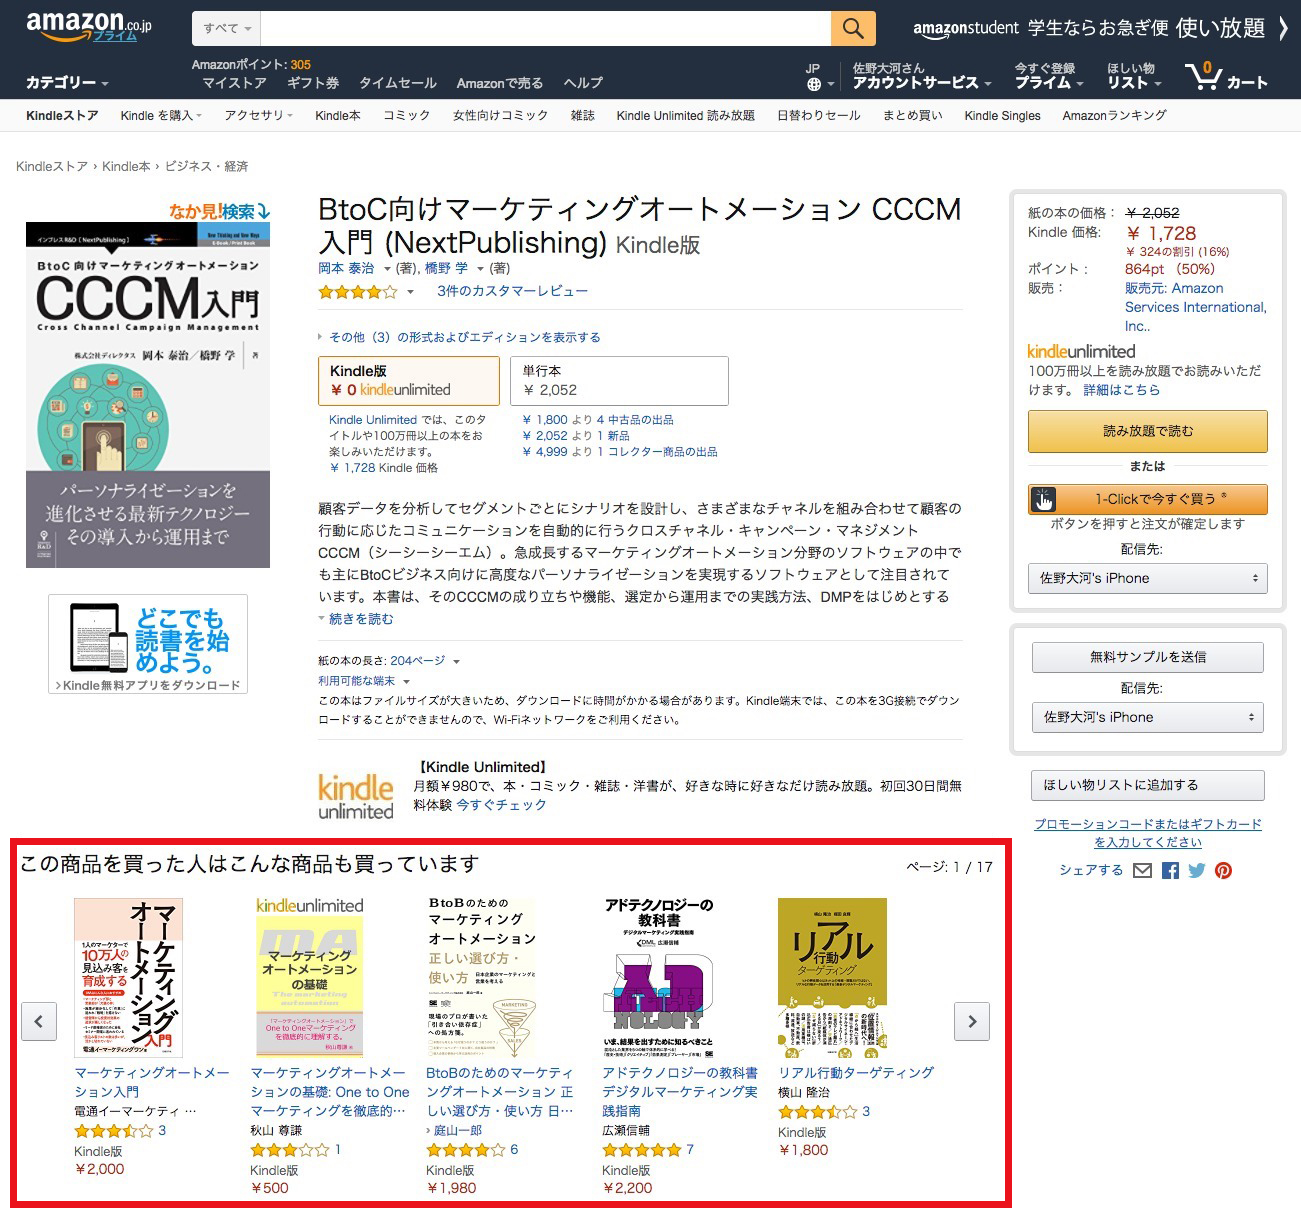
\includegraphics[width=0.8\hsize]{./images/research_amazon.jpg}
    \caption{Amazon 商品ページ}
    \label{fig:research-amazon}
  \end{center}
\end{figure}
\fi

\subsection{ユーザの位置情報を活用したパーソナライズ}
本研究と同じく,スマートフォンで得られるユーザの位置情報を活用したパーソナライズの事例を検討する.
% \subsubsection{行動ターゲティング広告}
様々な企業が提供するWeb広告の分野では,顧客ごとにパーソナライズされた広告を配信する行動ターゲティング広告の手法が行われ,近年では特に,ユーザの位置情報を活用したターゲティング広告に注目が集まっている.

% 株式会社博報堂DYメディアパートナーズ(以降,博報堂DYメディアパートナーズと表記),タメコ株式会社(以降,タメコと表記),デジタル・アドバタイジング・コンソーシアム株式会社(以降,DACと表記)の三社は,
博報堂DYメディアパートナーズ,タメコ,デジタル・アドバタイジング・コンソーシアム(以降,DACと表記)の三社は,生活者のリアル行動特性に基づき,パーソナライズされた広告配信を実現するメディアサービスの提供に向けた取り組みを実施している\cite{tameco}.
具体的には,タメコが持つ位置情報・動線情報の測量技術を用いて,博報堂DYメディアパートナーズがユーザの位置データとオンライン行動データを連携させ,個々人に応じた配信情報を自動化するメディアサービスを開発しDACが運営を行う.

広告配信サービスである「BitBlend(ビットブレンド)\cite{bitblend}」は,端末から得られる位置情報を活用し,ユーザの行動に応じた動画広告配信を行う.例えば,ある店舗への来店を促したい場合において,店の周辺にいるユーザを対象に,クーポンなどの店舗へ誘導するような広告を打つことで,費用対効果の高い施策が図れる.システムの概要を図\ref{fig:bitblend}に示す.

このように,企業が持つ顧客データや広告配信データに加え,ユーザの位置情報を組み合わせることで,ユーザの屋外での行動に応じてカスタマイズされた広告配信を実現可能としている.

% 位置情報を活用した広告配信方式には大きく分けて「リアルタイム方式」と「プロファイル方式」の2種類がある.リアルタイム方式では,GPSだけでなくBLEを使用したビーコンによる位置情報を用いて,店舗の周辺にいるユーザに対し割引クーポンを配信するなど,特定の範囲内にいるユーザをターゲットにした広告を配信する.
% プロファイル方式では,GPSの時系列的な蓄積情報から,ある時間帯に特定の場所によくいりことを割り出し(学生であることを割り出したり),新宿勤務者に対して新宿の店舗の広告を出すなど,ユーザに対し広告を配信する.
% (いらないかも)

% \subsubsection{ローカライズ検索}

Google検索エンジンのパーソナライズド検索では,検索時のユーザの位置情報に基づいて,表示内容や順位を切り替えるローカライズ検索という機能がある.弁護士,宅配といった地域依存性の高いサービスや,レストラン,カフェ,映画館といった施設に関するキーワードで検索した際に影響する.
例えば,ユーザが東京の渋谷区内で「カフェ」と検索した場合,検索結果には渋谷区周辺のカフェの情報やリンクが表示され,また,他の地域で検索した場合には別の検索結果が表示される(図\ref{fig:localize-search}).
ローカライズ検索には企業や店舗運営者にもメリットがあり,検索エンジンにおいて大手が独占していたキーワードでも,地域を特定すれば検索エンジンからの集客が見込めるようになる.

% 同じローカライズ検索でも,パソコンからの検索では県単位でのローカライズが見られるのに対し,スマートフォンからの検索では,端末のGPS機能を利用することで,より狭い地域でのローカライズが実現されている.

このように,オンライン上の行動データだけでなく,位置情報から得られるユーザのリアル行動データを用いたパーソナライズの事例がいくつかみられ,これらは,現代のユーザの多くが屋外でも常にスマートフォンを所持していることから実現できる事例だといえる.
しかしこれらのパーソナライズは,サービス利用時の一時的な位置情報を用いて,ユーザの現在地周辺にある情報の絞り込みや配信を行なっているため,
長期的に蓄積した位置情報から生活圏を検出し,各地域の情報を絞り込む本研究とは異なる.また,ユーザの位置情報をWeb上で扱うことからプライバシー保護の問題が懸念される.


\fifigure
\begin{figure}[H]
  \begin{center}
    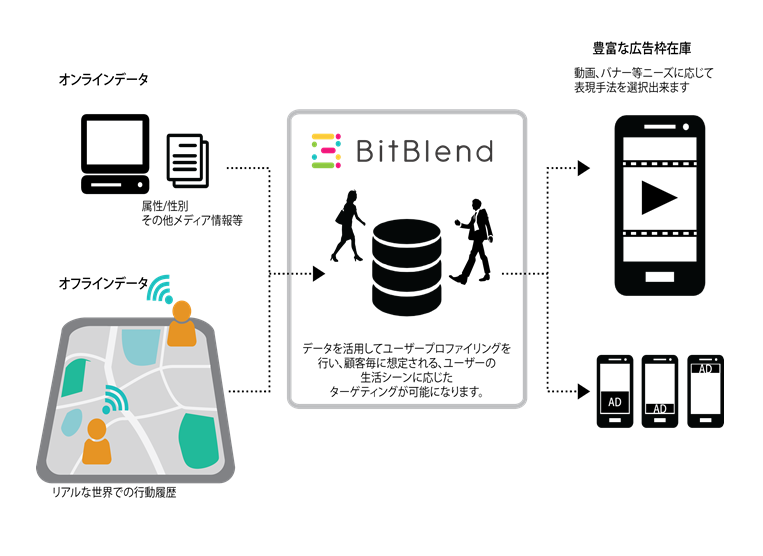
\includegraphics[width=0.85\hsize]{./images/bitblend.png}
    \caption{BitBlend 概要図}
    \label{fig:bitblend}
  \end{center}
\end{figure}
\fi

\fifigure
\begin{figure}[H]
  \begin{center}
    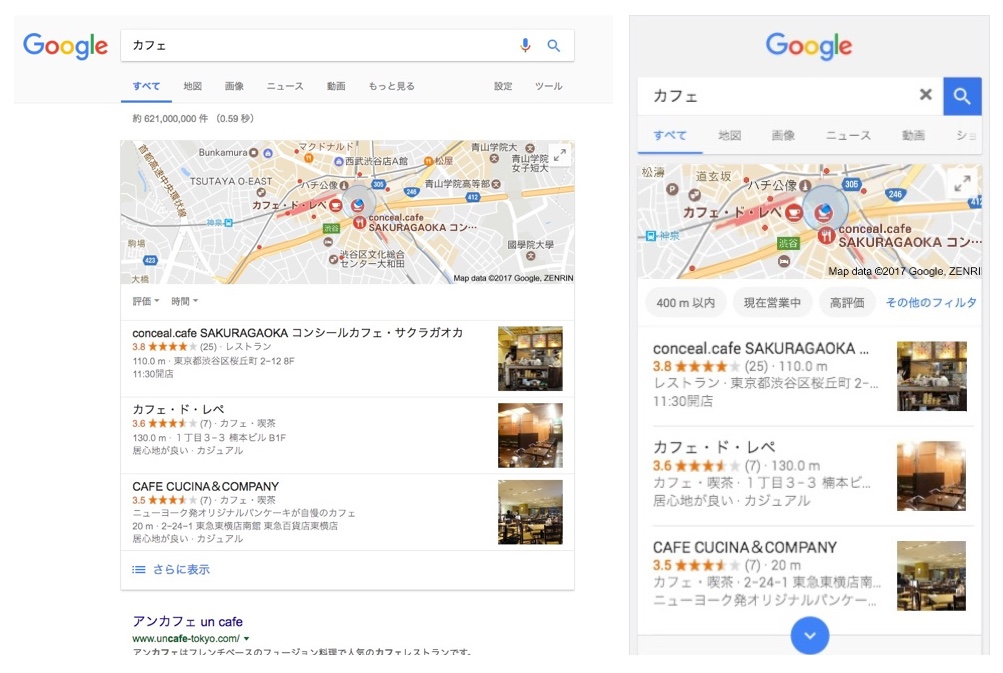
\includegraphics[width=0.85\hsize]{./images/localize_search.jpg}
    \caption{Google ローカライズ検索}
    \label{fig:localize-search}
  \end{center}
\end{figure}
\fi

\subsection{生活地域の選択によるコンテンツのカスタマイズ}
本研究と同じく,ユーザの生活圏に基づいたコンテンツのカスタマイズを行うサービスの事例を検討する.
「Yahoo!防災速報\cite{yahoo}」では,自身の生活地域を予めアプリに登録しておくことで,その地域で発生した災害情報を通知で受け取ることができる.
ユーザは自宅や実家,職場などが位置する地域を登録し,その地域で緊急地震速報や豪雨速報といった災害情報が発生した際に,一早く情報を受け取るという利用方法が想定される.(図\ref{fig:yahoo-watav}左)
% (前述で述べた事例のような,ユーザの興味関心を惹きつけるというより,必要度?に合わせたパーソナライズを行なっているみたいなことをいいたい)

% 東京都で起きた豪雨速報を,受け取りたい大阪住民は多くはいないだろう.てきな例文
% 興味関心を惹きつけるというより,緊急性,必要性の高い情報を個々に振り分け,カスタマイズしている.

イベントに特化したキュレーションアプリである「watav\cite{watav}」は,選択した都道府県エリアに合わせたイベント情報の絞り込みを行なっている.
アプリの初回起動時に選択したカテゴリや閲覧履歴を元に,ユーザの趣味嗜好に合わせたイベント情報のカスタマイズを行い.
加えてエリアによる絞り込みを行うことで,ユーザはイベント情報の中から「行きやすい場所」の情報を優先的に受け取ることができる.(図\ref{fig:yahoo-watav}右)

% 位置情報に紐づくイベント情報を扱うこのアプリに適しているといえる.

このように,スマートフォンの位置情報を利用せずユーザに生活地域を選択させ,コンテンツをカスマイズする手法の事例がいくつかみられる.
% ユーザは自身の生活地域の周囲に関する情報を優先的に受け取れるといったメリットがあり,これは本研究のにも共通する点であると考えられる.
こういった手法は地域依存性の高い情報を扱うサービスに適しており,これは本研究にも共通する点であると考えられる.
% Yahoo!防災速報のような緊急性の高い?情報や,watavのイベントといったエンターテイメント性のある情報など,分野を問わず適応できるといえる.
しかし,これらは生活圏の検出がユーザの選択で行われ,位置情報履歴から自動で生活圏を検出する本研究とは異なる.

\fifigure
\begin{figure}[H]
  \begin{center}
    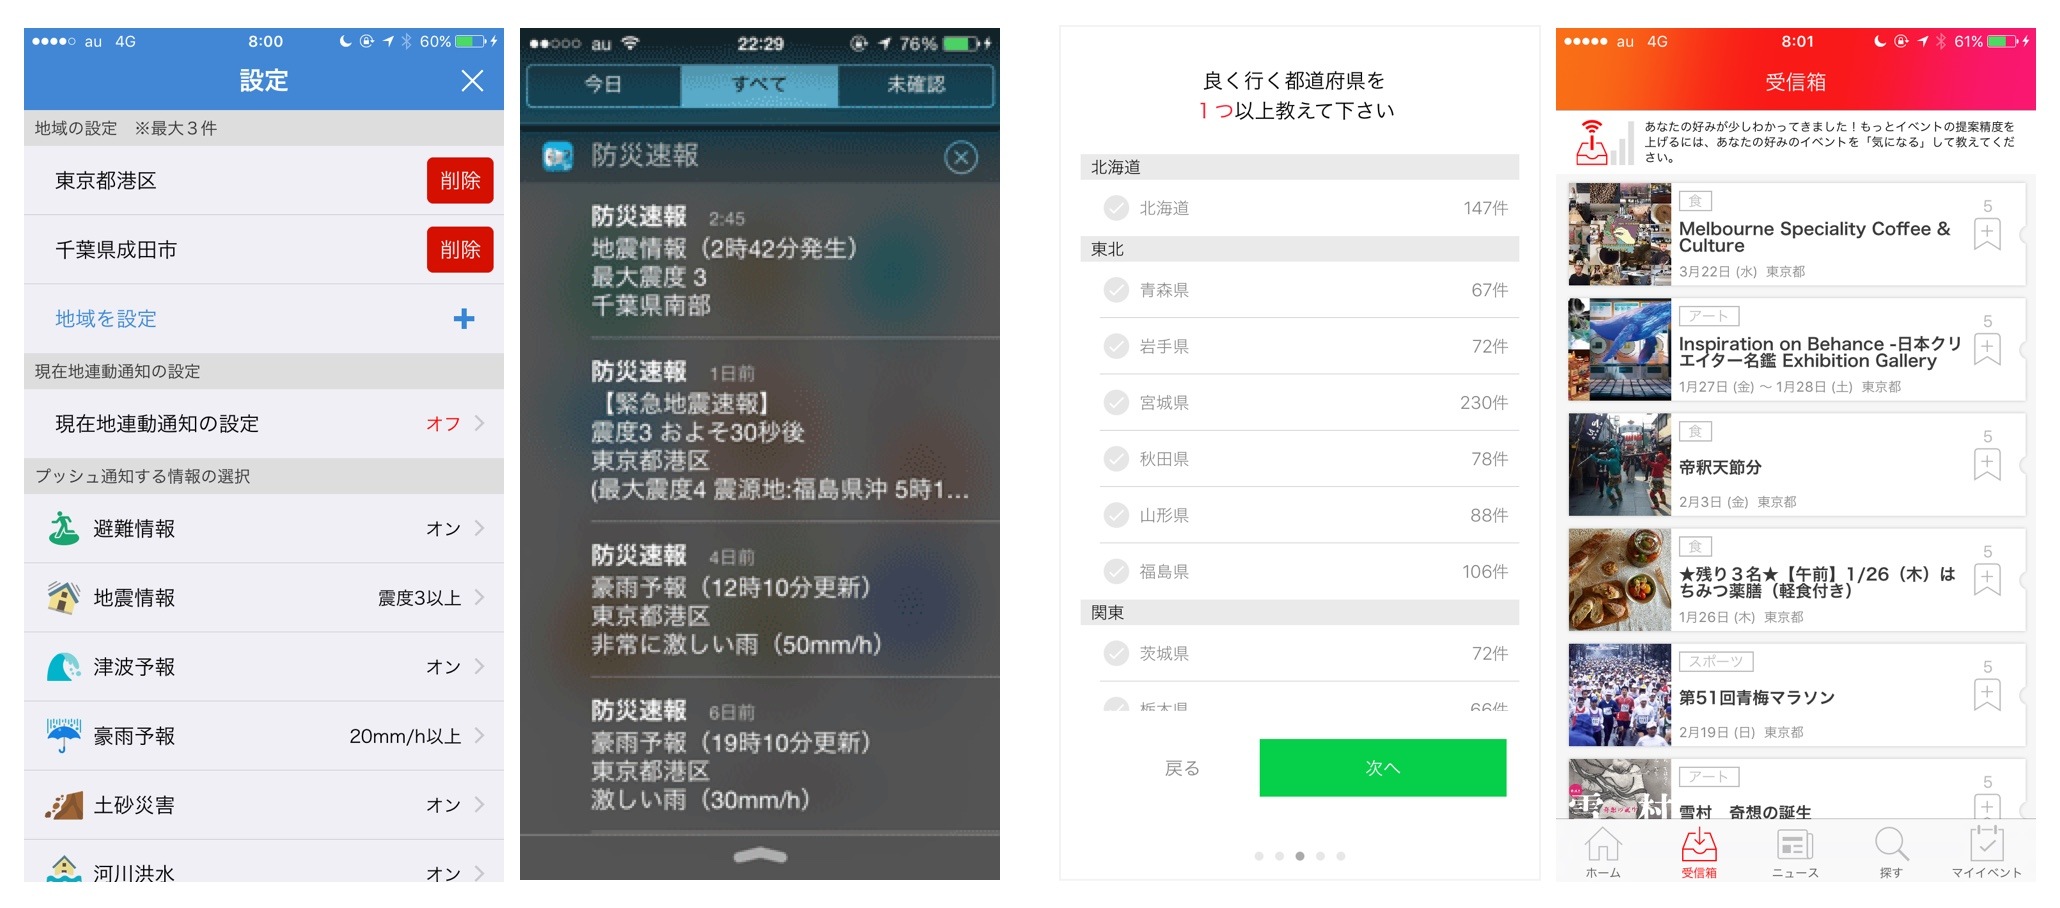
\includegraphics[width=1.0\hsize]{./images/yahoo_watav.jpg}
    \caption{左:Yahoo!防災速報,右:watav}
    \label{fig:yahoo-watav}
  \end{center}
\end{figure}
\fi


\subsection{位置情報履歴を用いた特性分析}
松尾らは,蓄積した位置情報からユーザの行動範囲を学習し,滞在地や経路を考慮した生活圏を検出する手法の研究を行なっている\cite{matsuo}.
滞在地の定義を「半径100m以内に連続で3分以上停留したGPSデータ群の重心点」とし,最も滞在頻度の多い場所を「自宅」,その他の滞在地と移動経路を結ぶ集合を生活圏として検出している.

宮崎らは,GPSにより得られる位置情報からユーザの滞在するエリアを識別し,高精度にユーザの行動を推定する方式を開発した\cite{docomo}.
推定に利用する位置情報を,単一データ(一組の緯度経度),系列データ(行動の開始から終了までの複数組の緯度経度),蓄積データ(長期間蓄積された複数組の緯度経度)に分類し,それぞれのデータからユーザの滞在エリアや移動経路,日常生活エリアといった情報を検出している.
日常生活エリア,即ちユーザの生活圏は,蓄積したエリア訪問の頻度から検出される滞在地域と,蓄積した移動経路から分析し検出される通勤・通学の経路で構成される.
% ユーザの日常生活エリアは,蓄積データから得られるエリア訪問の頻度や,移動経路の蓄積から示される通勤経路の算出によって推定している.
また,ユーザの現在の状況や行動パターンに応じて,各種サービスを高度化することが可能だと述べ,ユーザの行動に応じた自動対話サービスや,家族や友人間でアバターを通じて互いの行動状況を把握できるサービスといった例を上げている.しかしこれらは提案段階であり,行動推定技術を用いたサービスの評価実験は行われていない.

このように,蓄積した位置情報から,特定のエリアへの訪問頻度や経路データを分析することで,個人の生活圏や行動特性を導き出せることが先行研究から明らかになった.
また,日常の生活圏の中でも高頻度で訪れる滞在エリアの検出は,特定のエリア内の出現回数を算出することで実現可能であり,本研究にも適応できると考える.

% と「経路」に分けて捉える手法が多く,特に

% ライフログの話はここに入れてもいいかも
% このように広範な領域に渡る個人の活動を 記録する方法として「ライフログ」が提唱されている [廣 瀬 06] が,これらは記録を主としており,記録の利用手 法については,様々な検討されている過程である.


% \subsection{本研究の位置づけ}
% これらの関連研究を踏まえ,本研究の位置付けを行う
% Webサービスにおいてパーソナライズは,ユーザ体験を向上させる重要な役割!(具体的に)
% そして!
% ユーザのオンライン上での行動だけでなく,リアル行動に基づいた情報の絞り込みといったパーソナライズをすることで
% ユーザのライフスタイルに沿った??生活スタイル?
% サービス全体のユーザ体験向上や,効率よくマーケティングができること,などが測れることが分かった.
%
% パーソナライズによって絞り込む情報は
% 位置情報によって絞り込めるもの,実空間の情報と結びついた情報を扱っている.
%
% しかし,現状の位置情報を用いたサービスは,ユーザの現在地に基づくものばかり
% 一方,位置情報履歴からユーザの特性を割り出すことあ可能だが,
% 蓄積し,生活圏を割り出し,情報を絞り込む行程を一つのサービス内で実現した例は未だ存在しない.
% そこで筆者は,
%
% 既存の位置情報に基づく情報提供サービスとの差別化を図る
% 蓄積したことを協調
%
% 実際に一般ユーザへの評価をもとめ,その利用可能性を検証する!
%
% 蓄積した位置情報を用いて,自動で生活圏の算出,情報の選択を行うアプリケーションを開発し,検証を行うことに新規性を示す.
% 〜なところに新規性を示す
%
% 書いてわかったが,これらは全部先行研究一つ一つのまとめで言うから不必要!

\subsection{開発の方針}
先行研究・先行事例を踏まえ,本研究の開発の方針を定める.
% 筆者は,スマートフォンによって得た位置情報を端末内に蓄積し,生活圏を割り出すことによって,ユーザの周囲に溢れる情報の中から「生活圏に関する」情報を絞り込むことが可能であろうと予想する.
本研究の目的は,端末内に蓄積された位置情報履歴をもとに,ユーザの生活圏に基づくWebサービスのパーソナライズを行うシステム・スマートフォンアプリを開発し,その利用可能性を検討することである.
そのためにまず,スマートフォンに蓄積された位置情報からユーザの生活圏を検出するシステムを開発し,その精度を検証する.
宮崎らの日常生活エリアの推定技術\cite{docomo}を参考に,高頻度で訪れる特定のエリアをユーザの「生活圏」として検出する.尚,本システムにおいてユーザの移動経路は考慮しないものとする.
% (もう少しちゃんとした理由を.絞り込みを行うのに移動経路はなくていいと考える理由を)
また,プライバシー保護の問題を考慮し,取得した位置情報は端末内で管理しサーバやクラウドへはアップしないものとする.

開発したシステムを用いて,ユーザの生活圏に基づき,1. ハザードマップ,2. Webメディアの情報を絞り込んで提示するスマートフォンアプリをそれぞれ開発し,検証を行う.
% (アプリケーションで扱う情報は,地域依存性が高く絞り込みが行えるように十分に多様なコンテンツが望ましい,〜という話を入れるかどうか)
アプリの形式は,端末のGPSを利用するためのSDKが豊富であり,バックグラウンドでの位置情報取得が可能なネイティブアプリとする.
これは,ブラウザを通してインターネット上からアクセスするWebアプリに比べ,端末内でのデータの蓄積や管理,利用といった処理工程を実行し易いためでもある.
また今回は,2017年1月現在,国内のスマホートフォンの66\%のシェア率を持つiPhoneを対象にiOSアプリを開発する.

% 生活圏を算出するシステムはフレームワーク化し,その後のアプリケーション開発に組み込める形式にする.
% 生活圏に基づいて情報の絞り込みを行う

% アプリケーションで扱う情報は,地域依存性が高く,絞り込みが行えるように十分に多様なコンテンツが望ましいという考えから,
% それぞれの1節で述べていることが,選定した理由だからここでこう述べるのは違う

% 今回は,ハザードマップとWebメディアの二つの領域において,アプリケーションを開発し,
% 開発したアプリをユーザに利用してもらい,検証を行う.

% 本開発の目的は,端末内に蓄積された位置情報履歴から割り出されたユーザの生活圏を元に,ユーザの周囲に溢れる情報の中から生活圏に関する情報を絞り込み提示するサービスを実現することである.

% 個人情報利用に関するプライバシー保護の問題なども指摘され\cite{sample},
% 通信を行う際は暗号化,そうじゃなければローカルで使用することが求められる.
% 本開発では,蓄積したユーザの位置データはサーバークラウドへの通信は行わず,ローカルのデータベースで管理する



% 今回は,位置情報の処理,データベースのフレームワークが豊富であり,スマートフォンユーザの〜\%を占めるiPhoneを対象に,iOSで動作するものを開発
% 位置情報を割り出すシステムは,展開性を考え,ライブラリ化し,使いやすい形を目指す
% 開発環境は,Apple社が提供するiOSアプリ開発ツールであるxcodeを利用する.プログラミング言語はSwift3.0を使用する.

% 位置情報の取得,蓄積,生活圏の算出は,ライブラリとしてまとめ,二次利用しやすい形にする.(次の賞で?)


\section{生活圏を検出するシステムの開発}
本章では,端末内に蓄積させた位置情報から生活圏を検出するシステムの構成及び動作検証について述べる.

\subsection{システムの概要}
本システムは,一定間隔で位置情報を取得し,ジオコーディングAPIによって地名を取得しデータベースに格納する.その後データを集計し,多く登場する地名をユーザの「生活圏」として検出する.
本システムの構成の詳細について図\ref{fig:livingarea-diagram}に示す.
位置情報の取得は,端末のGPSやコンパスを扱うための機能が揃えられた,iOSのCore Location Frameworkを用いる.GPSが利用可能な場合には10m程度の誤差で,屋内などGPSが利用できない場合には,基地局からの電波取得により約300m単位のエリアで取得できる.データの蓄積や管理にはモバイル向けのデータベースであるRealmを用いる.位置情報は基本的にアプリがバックグランドにある状態で取得されることを想定し,得られたデータは一時的に位置情報を保存するデータベース(以降,DB1と表記)へと格納する.DB1のカラムは緯度,経度,日時で構成され,表\ref{tab:livingarea-db-1}のように定義する.

アプリがフォアグラウンドにきたタイミングで,DB1に蓄積されたデータを取り出し,GoogleのジオコーディングAPIを用いて各地点の地名を取得する.
市区町村などの地域名と,その下の1次的な下位地域名をそれぞれ取得し,緯度経度と日時のデータと併せ,長期的に位置情報・地名を保存するデータベース(以降,DB2と表記)へ格納する.DB2は表\ref{tab:livingarea-db-2}のように定義する.地名の取得及びDB2への追加が完了したタイミングでDB1の中身を削除する.
このように,位置情報の取得・保存,緯度経度からの地名の取得の行程を段階的に行うことで,バックグラウンドでのタスクを減らし,デバイスへの負担やシステムエラーといったリスクを低減させる.

次に,DB2のデータから,地域名と下位地域名を繋げた名称の出現数を算出し,データベース3(以降,DB3と表記)に格納する.この際,地域内に点在する緯度経度の重心位置を,緯度経度それぞれの平均値から算出し,併せて格納する.DB3は表\ref{tab:livingarea-db-3}のように定義され,出現数の値に従い降順に並び替える.
この結果,DB3で上位に現れる地域及び地点が,本システムの利用中にユーザが最も訪れたエリアであり,ユーザの生活圏だと考えられる.時間データを保持するDB2とDB3を別々で管理することで,指定した期間内のユーザの生活圏を検出することも可能である.

これらのデータは個々の端末内のみで保存・処理し,サーバやクラウドには共有されないようにする.このことによって,個人情報が漏洩するリスクを低減する.

本システムはこれらの一連の行程を自動で行い,別ファイルから必要に応じて生活圏データの取得が可能なメソッドを付け加え,後述するスマートフォンアプリに組み込めるフレームワークとして用意する.

\fifigure
\begin{figure}[H]
  \begin{center}
    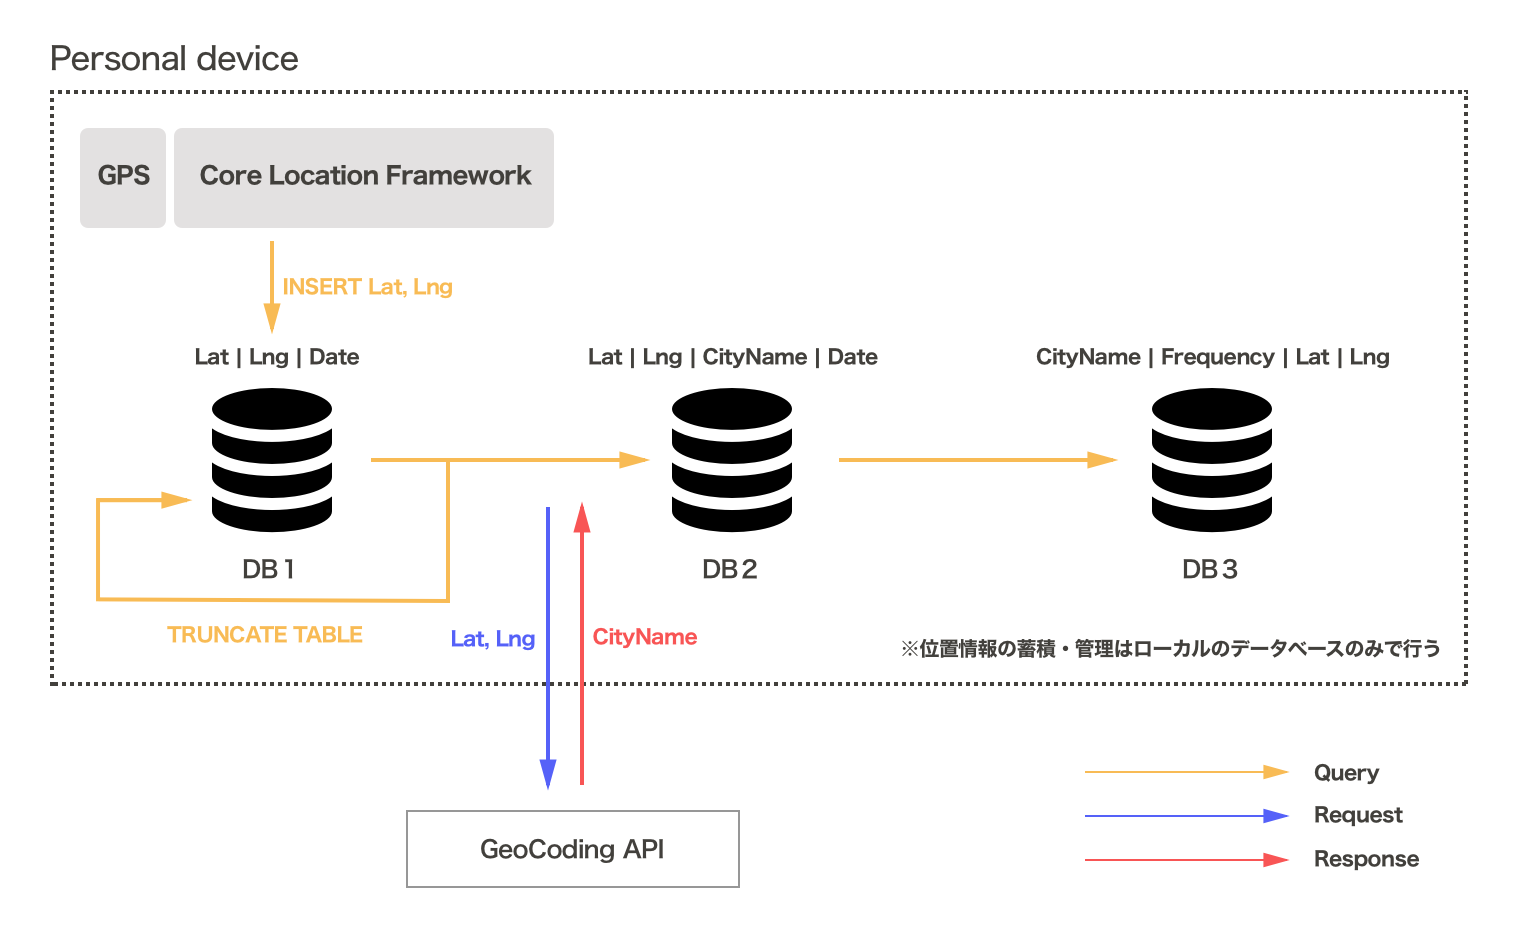
\includegraphics[width=1.0\hsize]{./images/livingarea_diagram.png}
    \caption{システム構成図}
    \label{fig:livingarea-diagram}
  \end{center}
\end{figure}
\fi

\begin{table}[H]
  \begin{center}
    \caption{一時的に緯度経度を保存するデータベース(DB1)のデータセット}
    \renewcommand\arraystretch{1.4}
    \begin{tabular}{|c|c|}
      \hline
      \multicolumn{1}{|c}{属性情報} & \multicolumn{1}{|c|}{ データ型 } \\
      \hline
      \hline
      \multicolumn{1}{|c}{緯度} & \multicolumn{1}{|c|}{Double} \\
      \hline
      \multicolumn{1}{|c}{経度} & \multicolumn{1}{|c|}{Double} \\
      \hline
      \multicolumn{1}{|c}{ 緯度軽度を取得した日時 } & \multicolumn{1}{|c|}{Date} \\
      \hline
    \end{tabular}
    \label{tab:livingarea-db-1}
  \end{center}
\end{table}

\begin{table}[H]
  \begin{center}
    \caption{長期的に位置情報・地名を保存するデータベース(DB2)のデータセット}
    \renewcommand\arraystretch{1.4}
    \begin{tabular}{|c|c|}
      \hline
      \multicolumn{1}{|c}{属性情報} & \multicolumn{1}{|c|}{ データ型 } \\
      \hline
      \hline
      \multicolumn{1}{|c}{緯度} & \multicolumn{1}{|c|}{Double} \\
      \hline
      \multicolumn{1}{|c}{経度} & \multicolumn{1}{|c|}{Double} \\
      \hline
       緯度軽度を取得した日時  & Date \\
      \hline
      地域名 & String \\
      \hline
      一次的な下位地域名 & String \\
      \hline
    \end{tabular}
    \label{tab:livingarea-db-2}
  \end{center}
\end{table}

\begin{table}[H]
  \begin{center}
    \caption{地名と出現数のデータベース(DB3)のデータセット}
    \renewcommand\arraystretch{1.4}
    \begin{tabular}{|c|c|}
      \hline
      属性情報 &  データ型  \\
      \hline
      \hline
      地域名 & String \\
      \hline
       下位地域名  & String \\
      \hline
      出現数 & Int \\
      \hline
      重心の緯度 & Double \\
      \hline
      重心の経度 & Double \\
      \hline
    \end{tabular}
    \label{tab:livingarea-db-3}
  \end{center}
\end{table}

\subsection{精度の検証}
前節で述べたフレームワークを用いて,検出された生活圏の地名を画面上に表示する実験用のアプリを開発する.複数のユーザを対象に動作実験を行い,システムの精度を検証する.

アプリの画面上には,使用期間内に一番訪れたと検出される地域上位4つの地名が表示される(図\ref{fig:system-ui}).被験者17名にアプリをインストールしてもらい,2〜3週間後にWebアンケートを実施する.アンケートの項目は表\ref{tab:system-test-content}の通りである.また,被験者の属性を表\ref{tab:system-test-userstatus}に示す.

\fifigure
\begin{figure}[H]
  \begin{center}
    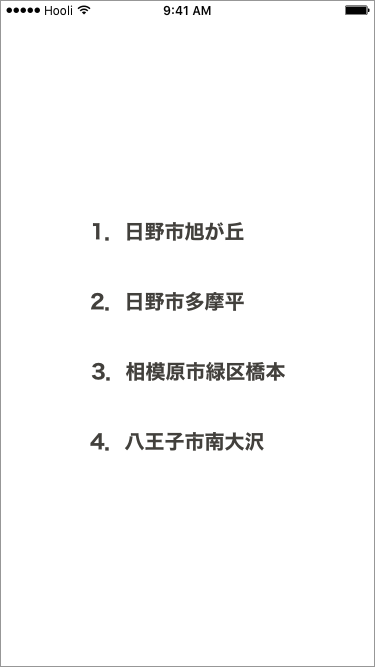
\includegraphics[width=0.4\hsize]{./images/system.png}
    \caption{実験用のアプリ画面}
    \label{fig:system-ui}
  \end{center}
\end{figure}
\fi

\begin{table}[H]
  \begin{center}
    \caption{アンケートの内容}
    \renewcommand\arraystretch{1.2}
    \begin{tabular}{|c|l|}
      \hline
      設問 & \multicolumn{1}{p{12cm}|}{アプリで提示されている場所は、普段生活している場所と一致していましたか} \\
      & 1.全て一致している \\
      & 2.時々違うことがあるがだいたい一致している \\
      & 3.一致していない場所が含まれてることが多い \\
      & 4.全く一致していない \\
      & 5.その他 \\
      \hline
    \end{tabular}
    \label{tab:system-test-content}
  \end{center}
\end{table}

\begin{table}[H]
  \begin{center}
    \caption{被験者の属性}
    \renewcommand\arraystretch{1.4}
    \begin{tabular}{|c|c|c|c|c|c|c|}
      \hline
      \multicolumn{1}{|l|}{回答者数} & \multicolumn{6}{c|}{17名} \\
      \hline
      性別 & \multicolumn{3}{c|}{男性} & \multicolumn{3}{c|}{女性} \\
      \cline{2-7}
      & \multicolumn{3}{c|}{16名} & \multicolumn{3}{c|}{1名} \\
      \hline
      年代 & 20代未満 & 20代 & 30代 & 40代 & 50代 & 60代以降 \\
      \cline{2-7}
      & 0名 & 8名 & 2名 & 5名 & 1名 & 1名 \\
      \hline
      職業 & 公務員 & 会社員・自営業 & 研究者 & 学生 & その他 &  \\
      \cline{2-7}
      & 1名 & 5名 & 0名 & 5名 & 6名 & \\
      \hline
    \end{tabular}
    \label{tab:system-test-userstatus}
  \end{center}
\end{table}

男性が多いという偏りはあるものの,様々な年代・職種の被験者が集まり,多様な移動パターンを揃えたといえる.
結果のグラフを図\ref{fig:system-result}に示す.

\fifigure
\begin{figure}[H]
  \begin{center}
    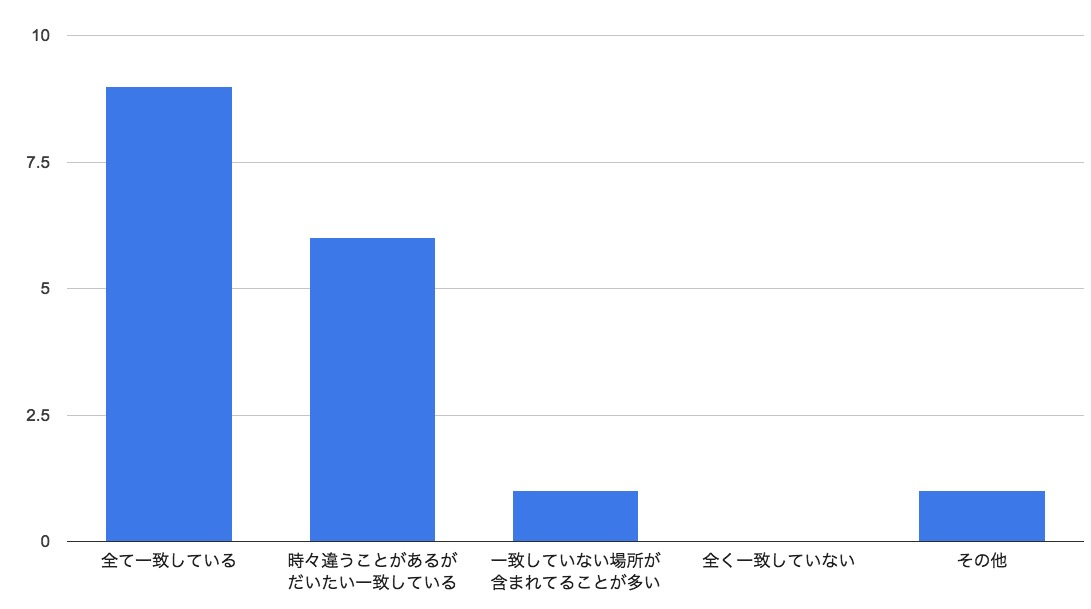
\includegraphics[width=0.9\hsize]{./images/system_result.jpg}
    \caption{アンケート結果(生活圏検出の精度の調査)}
    \label{fig:system-result}
  \end{center}
\end{figure}
\fi

アンケート調査の結果「アプリで提示されている場所は、普段生活している場所と一致していましたか」という設問に対して,被験者17名中9人が.「全て一致している」と回答した.また「時々違うことがあるがだいたい一致している」と回答した人は6名であり,全体の88\%の被験者に対し,高い精度で生活圏を検出できたといえる.
一方「一致していない場所が含まれてることが多い」と回答した人が1名,「その他」を回答した人が1名であり,その内容は「移動しすぎて安定しない」であった.
二人の被験者はどちらも20代の学生であることから大学生と予想でき,他の職種に比べて移動パターンの統一性が低いことからこのような結果になったと考えられる.
しかし「全く一致していない」と回答した人は0名であり,また,被験者の過半数が高い精度で生活圏を検出できていたことから,筆者が用いた手法は適切であり,本システムの精度は十分であるといえる.




\section{ハザードマップアプリにおけるパーソナライズ}
本章では,前章で述べたシステムを組み込み,検出された生活圏をもとにハザーマップの情報を絞り込んでユーザに提示するスマートフォンアプリの仕様と実装について述べる.
さらに,実証実験とアプリ公開後にそれぞれ実施したアンケート調査の結果と考察について述べる.
% まず,ハザーマップアプリの概要と既存の課題を整理し,開発の方針を定める.次いで,利用データとシステム・画面の構成について紹介する.
% 鎌倉市で行われた実証実験での活用と,アプリの一般公開の後ユーザを対象に実施したユーザの評価を元に,位置情報履歴から割り出された生活圏を元にパーソナライズを行う本アプリの利用可能性を示す.

\subsection{ハザードマップアプリの概要と開発の目的}
ハザードマップアプリとは,災害時の被害範囲・程度,避難施設等を図示したハザードマップを,端末で閲覧できるようにしたアプリである.
近年多くの企業や自治体が開発・配布を行い,2016年10月現在,App Storeにおいて防災に関連するアプリは200以上ある.
% スマートフォンの普及と,国内におけるオープンデータの推進によりGIS関連のアプリが誰でも作成できようになり,
% 2016年10月現在,App Storeにおいて防災に関連するアプリは200以上あり,また地域の自治体によって作成されたアプリは70ほど存在している.
一般的にハザードマップは,災害時の利用や,防災のための事前学習,地域の災害訓練などで活用される.
しかし,アプリとしてハザードマップを簡単に利用できる一方,画面サイズに対して情報量が多く,閲覧性や操作性が低いという課題が考えられる.
また,ハザードマップアプリは自治体ごとに地域のデータをまとめて作られている場合が多く,隣接する地域や,その他の地域の状況を知るには別途他のアプリで情報を収集しなけれならない.

そこで筆者は,全国のハザードマップの情報から,ユーザの生活圏に基づいて情報を収集し提示することで,既存のアプリの閲覧性や情報収集における課題を解決できると予想する.
尚本アプリは,災害時ではなく,平常時に災害のリスクや避難施設といった防災情報について,事前に学習することを目的に使用することを想定する.


\subsection{アプリケーションの概要}

\subsubsection{利用データの設計}
本アプリで用いる全国のハザード情報のデータ設計及びAPIの仕様について述べる.
日本国内には行政や地方自治体が提供する,二次利用可能な形で公開されたGISオープンデータが多数存在する.
% ここで,二次利用可能な形とは,二次利用可能な利用ルールが整備されかつJSONやXMLなど機械判読に適したデータ形式であることをいう.
本開発では,国土交通省国土政策局国土情報課の国土数値情報\footnote{http://nlftp.mlit.go.jp/ksj/}の避難施設,浸水想定区域,土砂災害警戒区域のオープンデータを用いる.
データをアプリ開発で扱い易い形式するため,XMLで書き出された各防災情報のオープンデータを,それぞれのデータセットで定義されたデータベースに格納する.さらに,緯度軽度を指定したリクエストを送ることで,緯度経度が指す地点から一定範囲内に含まれる防災データのレスポンスが帰ってくる独自のAPIを実装する.これに防災科学技術研究所\footnote{http://www.j-shis.bosai.go.jp/}が提供する地震ハザード情報提供APIを加え,本アプリに組み込み開発を行う.
各防災データの概要について以下に記載する.

\begin{itemize}
  \item 避難施設データ

  災害対策基本法に基づき都道府県及び市町村により作成された地域防災計画に示される避難施設のデータ.
  データセットは表\ref{tab:database-facility}のように定義する.

  \item 浸水想定区域データ

  河川管理者から提供された浸水想定区域図を製品仕様に基づき浸水深ごとのポリゴンデータとして整備したもの.
  データセットは表\ref{tab:database-flood}のように定義する.

  \item 土砂災害警戒区域データ

  都道府県が指定する土砂災害警戒区域の範囲または位置,及び種別,名称等のデータをポリゴンデータとして整備したもの.
  データセットは表\ref{tab:database-sediment}のように定義する.

  \item 地震ハザードステーション 地震ハザード情報提供API
  指定した250mメッシュの30年震度5弱以上/5強以上/6弱以上/6強以上となる確率等,J-SHIS地点情報で出力可能な地震ハザード属性を提供する.

\end{itemize}

\begin{table}[H]
  \begin{center}
    \caption{避難施設データセットの定義}
    \renewcommand\arraystretch{1.4}
    \begin{tabular}{|c|c|c|}
      \hline
      属性情報 & データ型 \\
      \hline
      \hline
      避難施設の位置 &  Geometry(点型)  \\
      \hline
      避難施設の名称 & String \\
      \hline
      避難施設の住所 & String \\
      \hline
      避難施設の種類 & String \\
      \hline
       避難施設の形態ごとの収容可能人数  & Int \\
      \hline
      避難施設の形態ごとの面積 & Int  \\
      \hline
    \end{tabular}
    \label{tab:database-facility}
  \end{center}
\end{table}

\begin{table}[H]
  \begin{center}
    \caption{浸水想定区域データセットの定義}
    \renewcommand\arraystretch{1.4}
    \begin{tabular}{|c|c|c|}
      \hline
      属性情報 & データ型 \\
      \hline
      \hline
       浸水想定区域の範囲(面)  & Geometry(面型) \\
      \hline
      浸水深 &  Int(浸水深のコードリスト型) \\
      \hline
    \end{tabular}
    \label{tab:database-flood}
  \end{center}
\end{table}

\begin{table}[H]
  \begin{center}
    \caption{土砂災害警戒区域データセットの定義}
    \renewcommand\arraystretch{1.4}
    \begin{tabular}{|c|c|c|}
      \hline
      属性情報 & データ型 \\
      \hline
      \hline
      土砂災害警戒区域(面) & Geometry(面型) \\
      \hline
      土砂災害警戒区域の現象の種類 & Int(急傾斜地の崩壊,土石流,地滑り)\\
      \hline
      土砂災害警戒区域の指定の種類 & Int \\
      &  土砂災害警戒区域(指定済) 土砂災害特別警戒区域(指定済)  \\
      & 土砂災害警戒区域(指定前) 土砂災害特別警戒区域(指定前) \\
      \hline
    \end{tabular}
    \label{tab:database-sediment}
  \end{center}
\end{table}

\subsubsection{画面構成・システム構成}
本アプリは,ユーザの生活圏に基づいて,全国のハザード情報を絞り込み提示をするハザードマップアプリである.ユーザの生活圏と現在地のボタンを表示するトップ画面(図\ref{fig:screen-structure-01}左)と,各防災情報を地図や数値で示す画面(図\ref{fig:screen-structure-01}右,図\ref{fig:screen-structure-02})で構成される.


\begin{enumerate}
  \item トップ画面

  アプリの起動時に,ローカルのデータベースからユーザの生活圏データを取り出し,上位四つの地名と,画像を並べたボタンを配置する.この画像は,Google Street View Image APIを用いて,指定した緯度経度からGoogleストリートビューの静的なパノラマ画像を取得し使用している.また,四つの生活圏のボタンに加え,上部に現在地のボタンも配置する.
  % ユーザに知っているであろう場所の風景写真を定時することで,パーソナライズを高めている的なこと,先行研究から言えたらいいな
  ボタンを選択した後,それぞれの地域における防災情報画面へ遷移する.
  % 防災情報画面の前に,ボタンが大きく配置されるこの画面を挟むことで,導線を明確にしている
  これによりユーザは,全国のハザード情報の中から,自身の生活圏内の防災情報に素早くアクセスし閲覧することができる.

  \item 防災情報画面

  防災情報画面は,上部のマップと,下部の防災情報に応じてグラフや数値を表示するビューで構成され,画面下の四つのアイコンから防災情報を切り替えられる.初回読み込みと切り替わりのタイミングで,前節で述べたAPIを用いて緯度軽度を指定したリクエストを送り,レスポンスとして防災情報を受け取る.さらに,データに応じて地図上にポリゴンやピンを配置し,数値や現象の種類といった情報示す.
  防災情報は中心点から半径5km以内に含まれる情報を取得・表示し,地図のドラッグにより中心点が範囲外に出た時にデータの再読み込みを行う.これにより,ユーザは自身の生活圏内またはその周りの地域の災害リスクや緊急時の避難施設について学習できる.
  % アイコンをタブの切り替えにした理由〜〜〜
\end{enumerate}


\fifigure
\begin{figure}[H]
  \begin{center}
    \begin{tabular}{ccc}
    \begin{minipage}{0.3\hsize}
	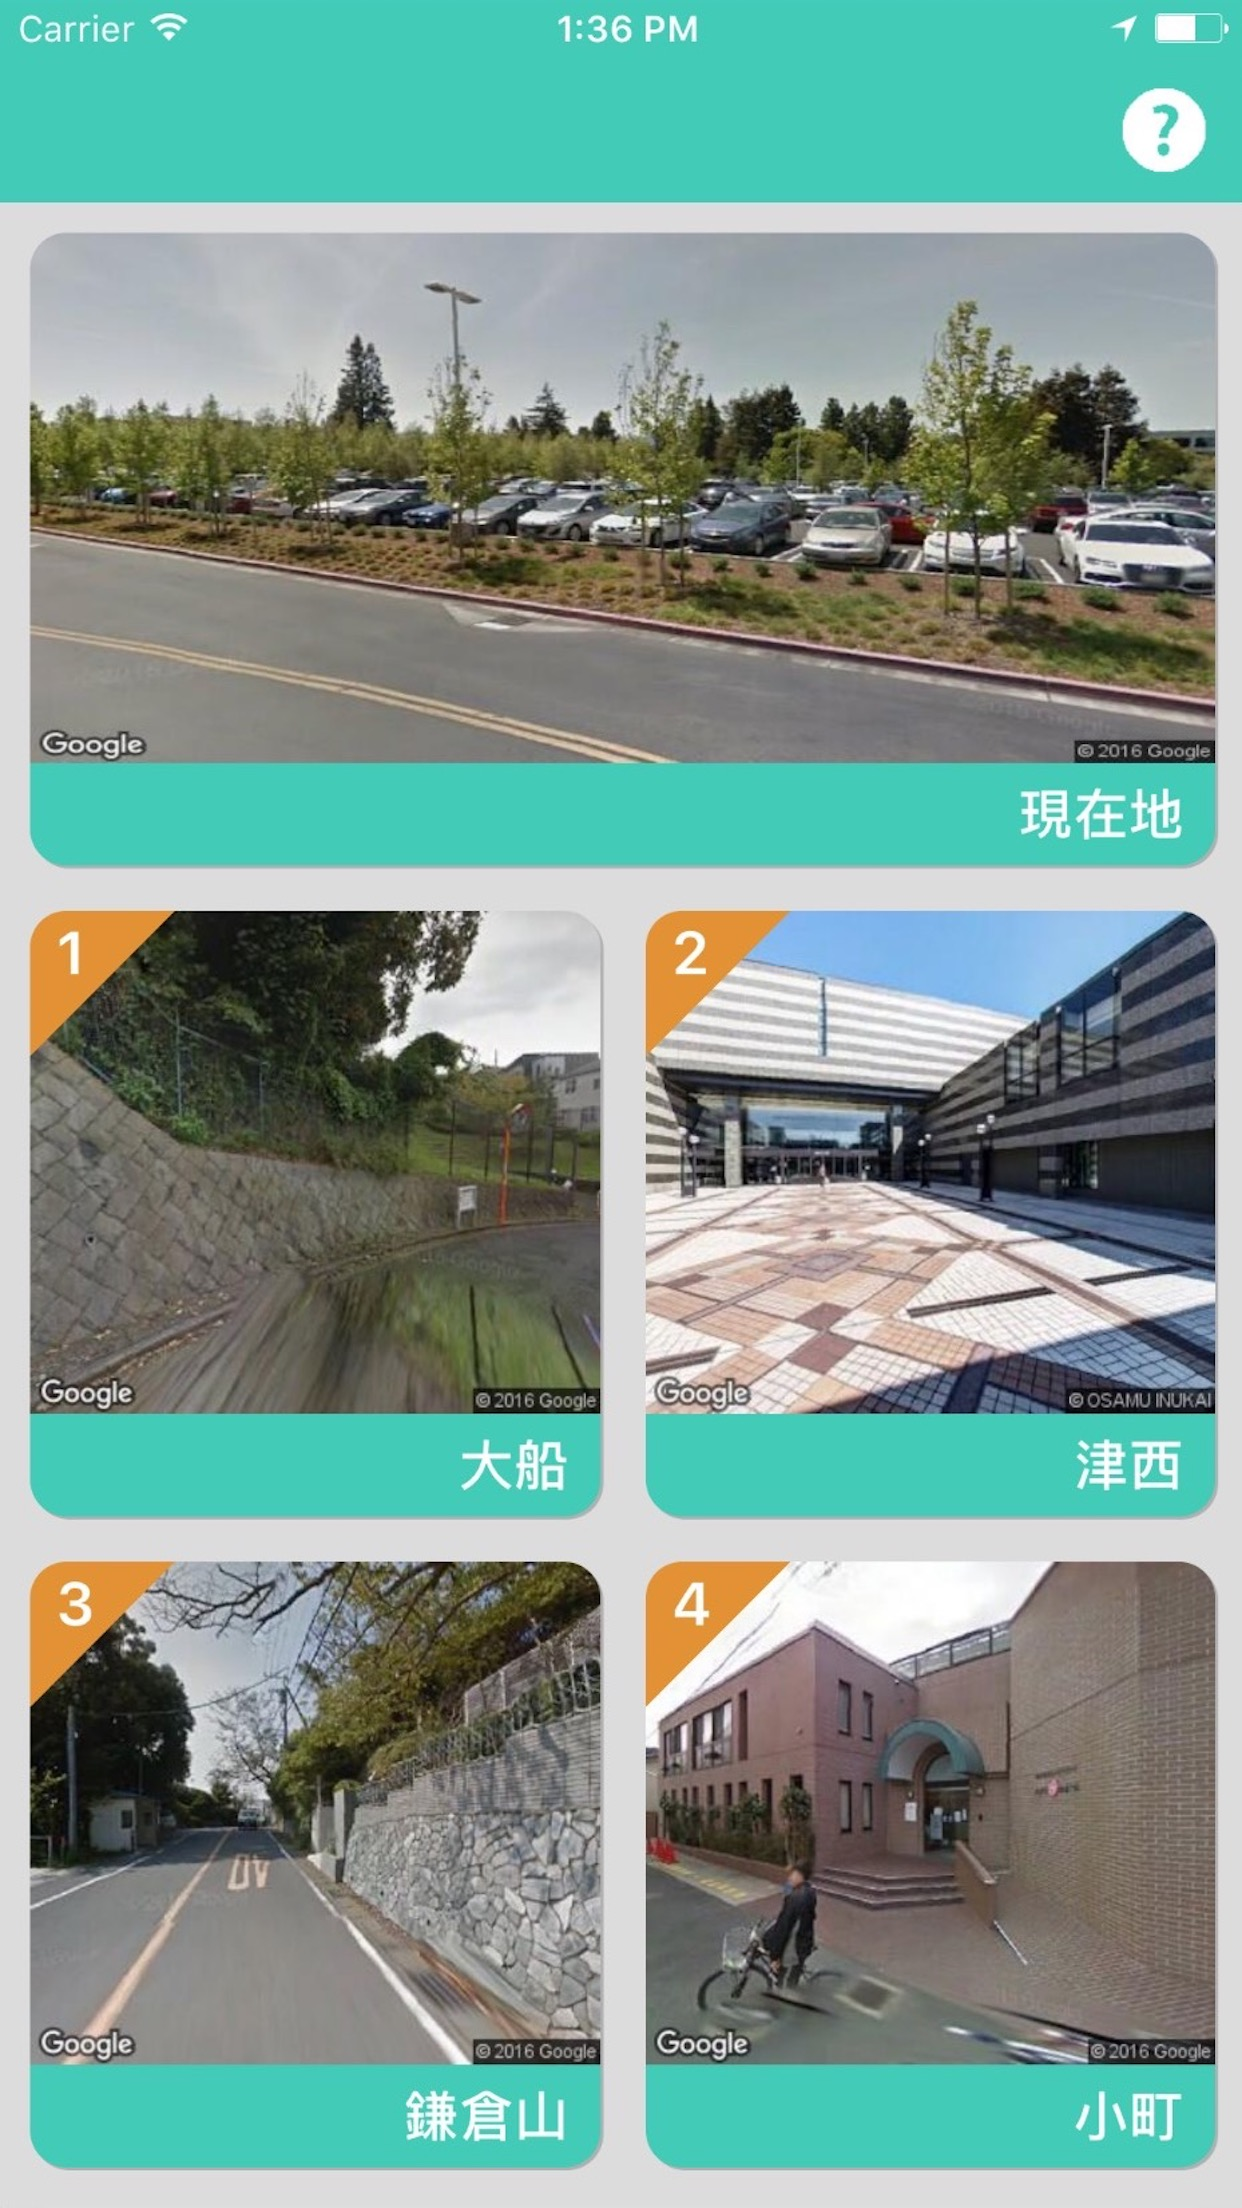
\includegraphics[width=\hsize]{./images/mbs_top.jpg}
    \end{minipage}
    &
    \begin{minipage}{0.3\hsize}
      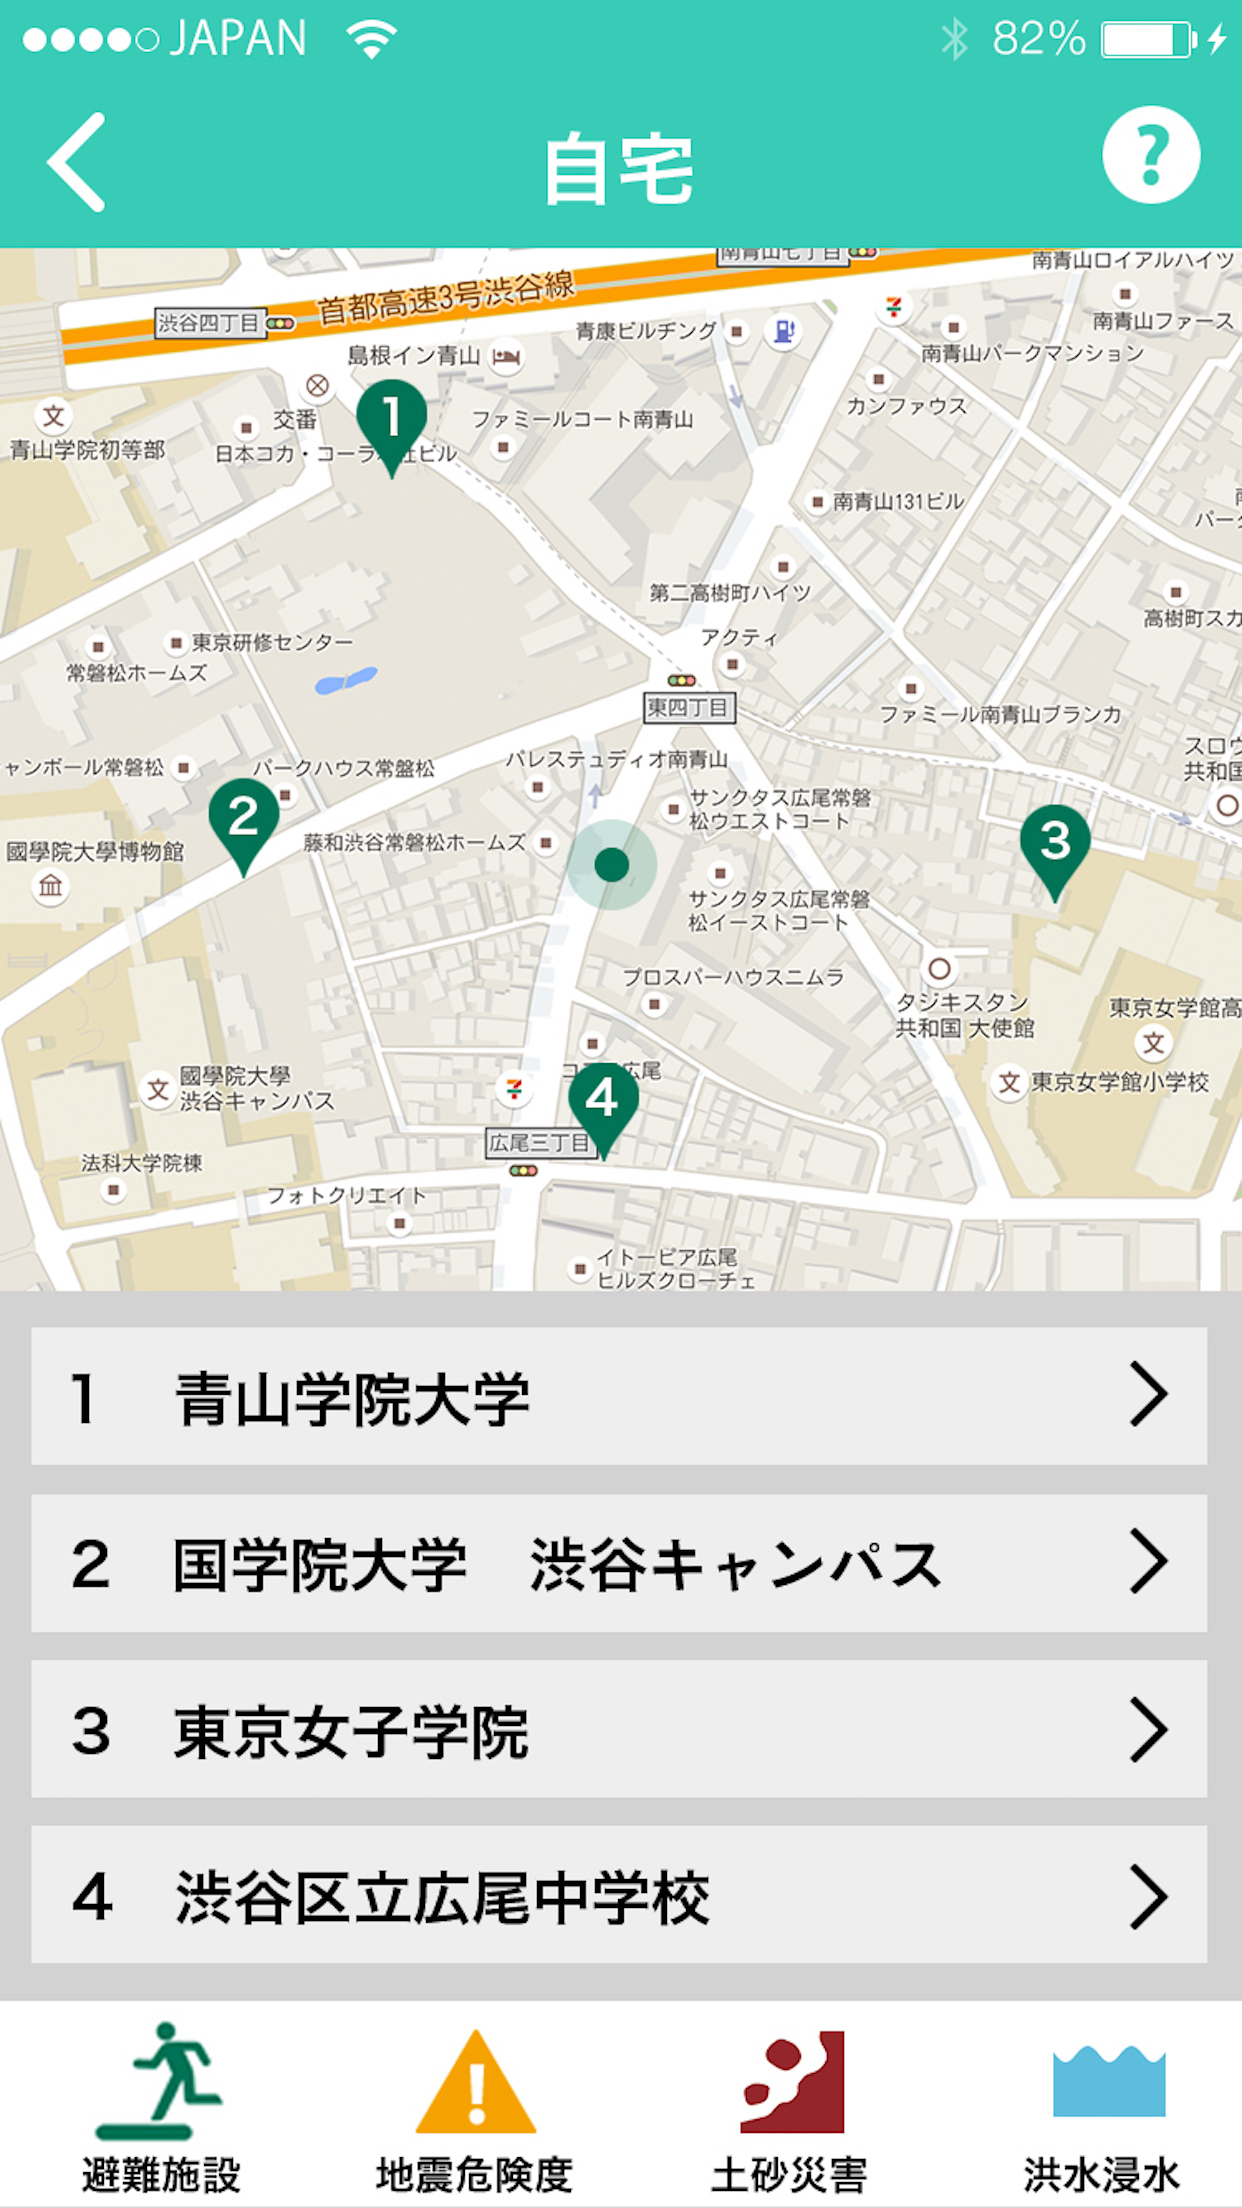
\includegraphics[width=\hsize]{./images/mbs_facility.jpg}
    \end{minipage}
  \end{tabular}
    \caption{左:トップ画面,右:防災情報画面(避難施設)}
    \label{fig:screen-structure-01}
  \end{center}
\end{figure}
\fi

\fifigure
\begin{figure}[H]
  \begin{center}
    \begin{tabular}{ccc}
    \begin{minipage}{0.3\hsize}
	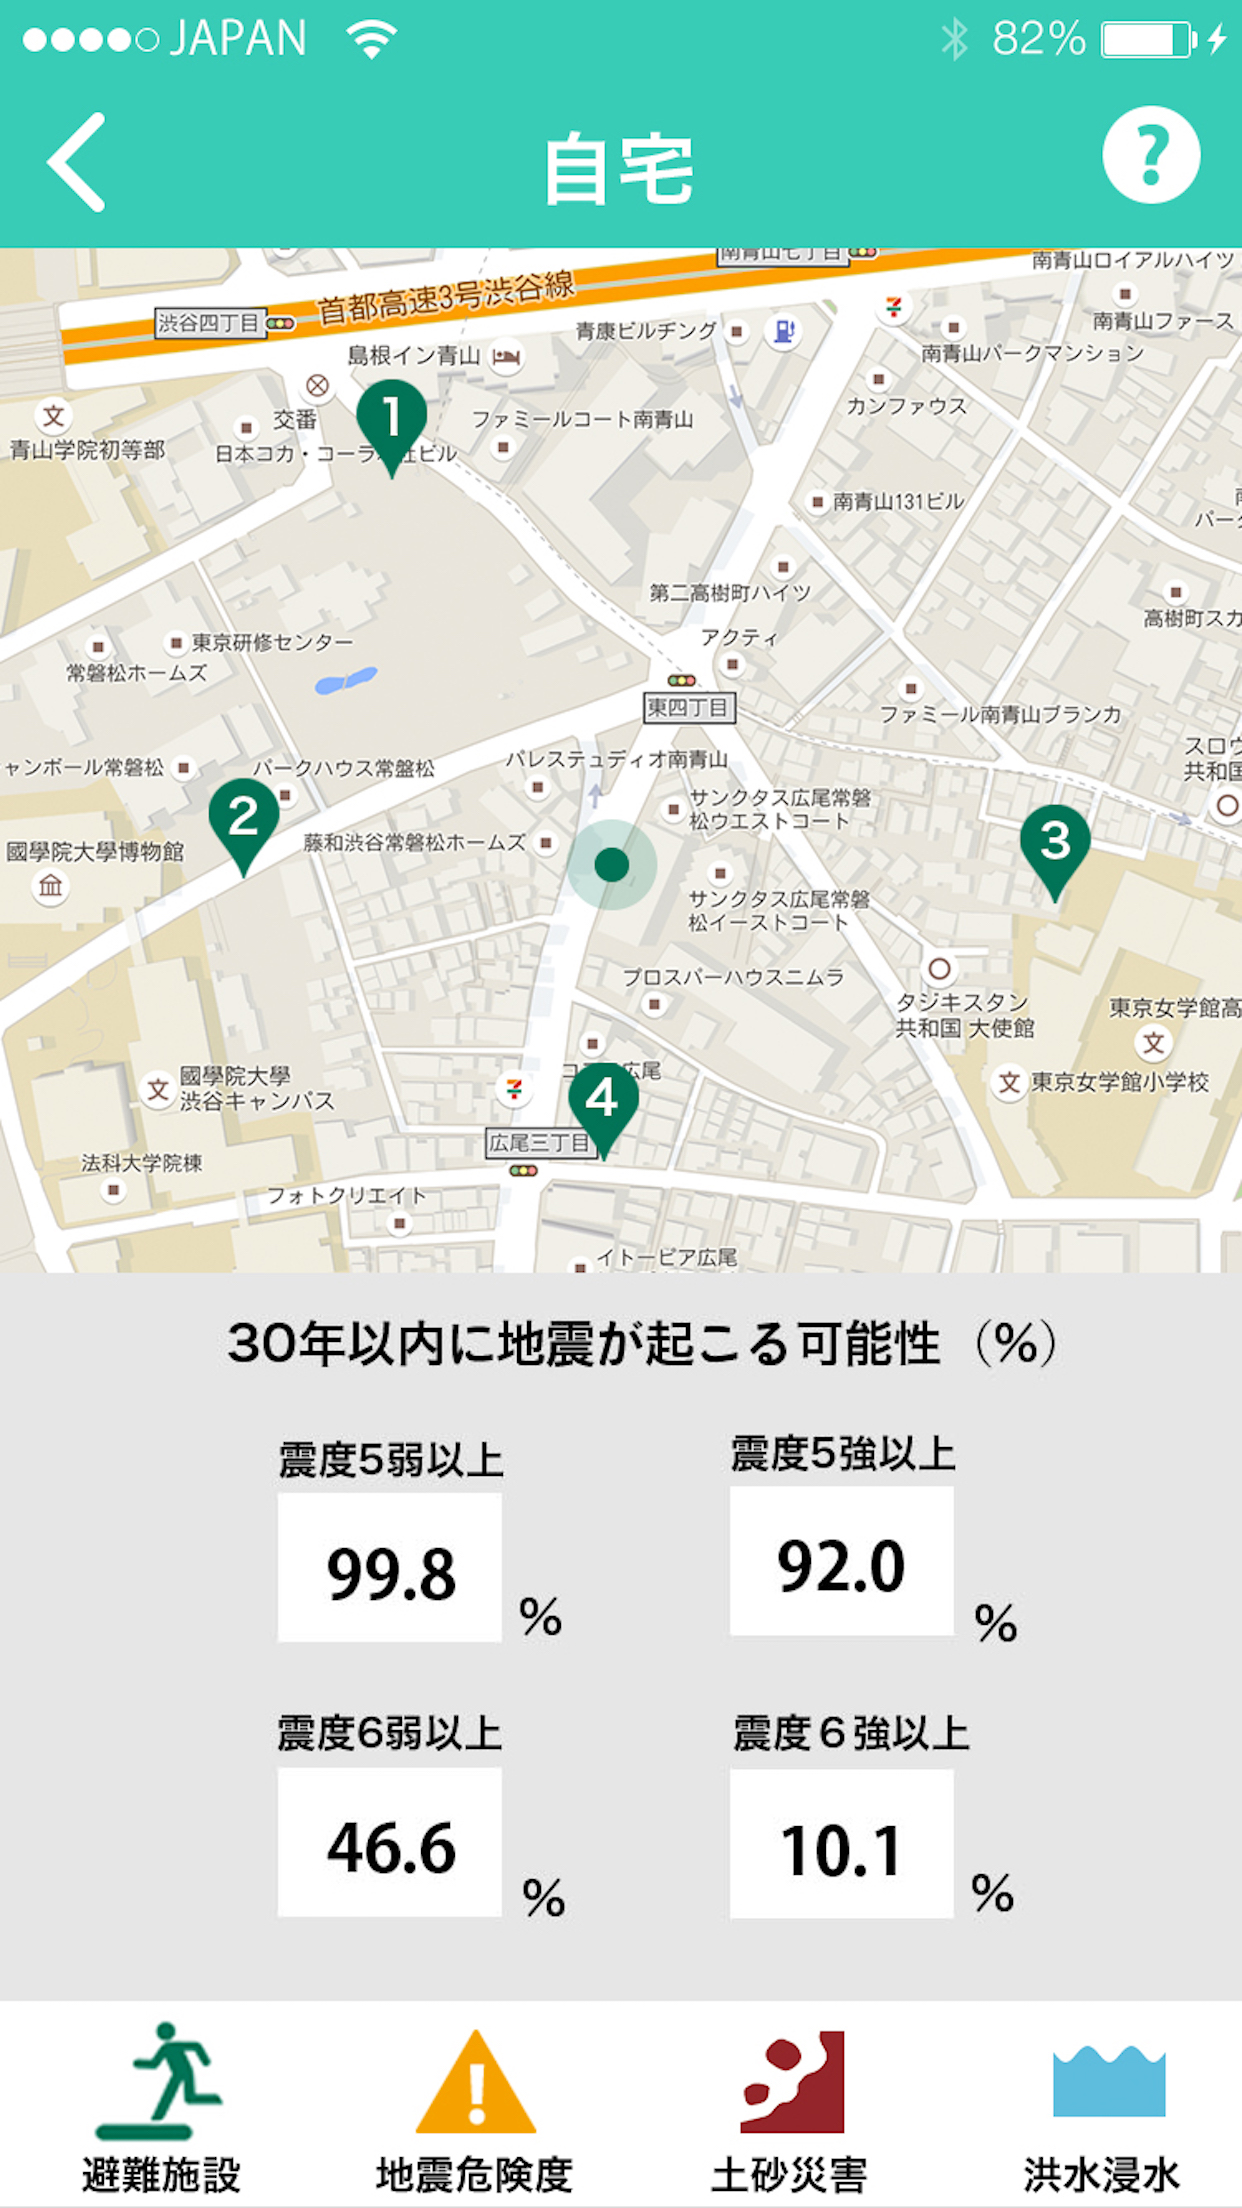
\includegraphics[width=\hsize]{./images/mbs_eq.jpg}
    \end{minipage}
    &
    \begin{minipage}{0.3\hsize}
      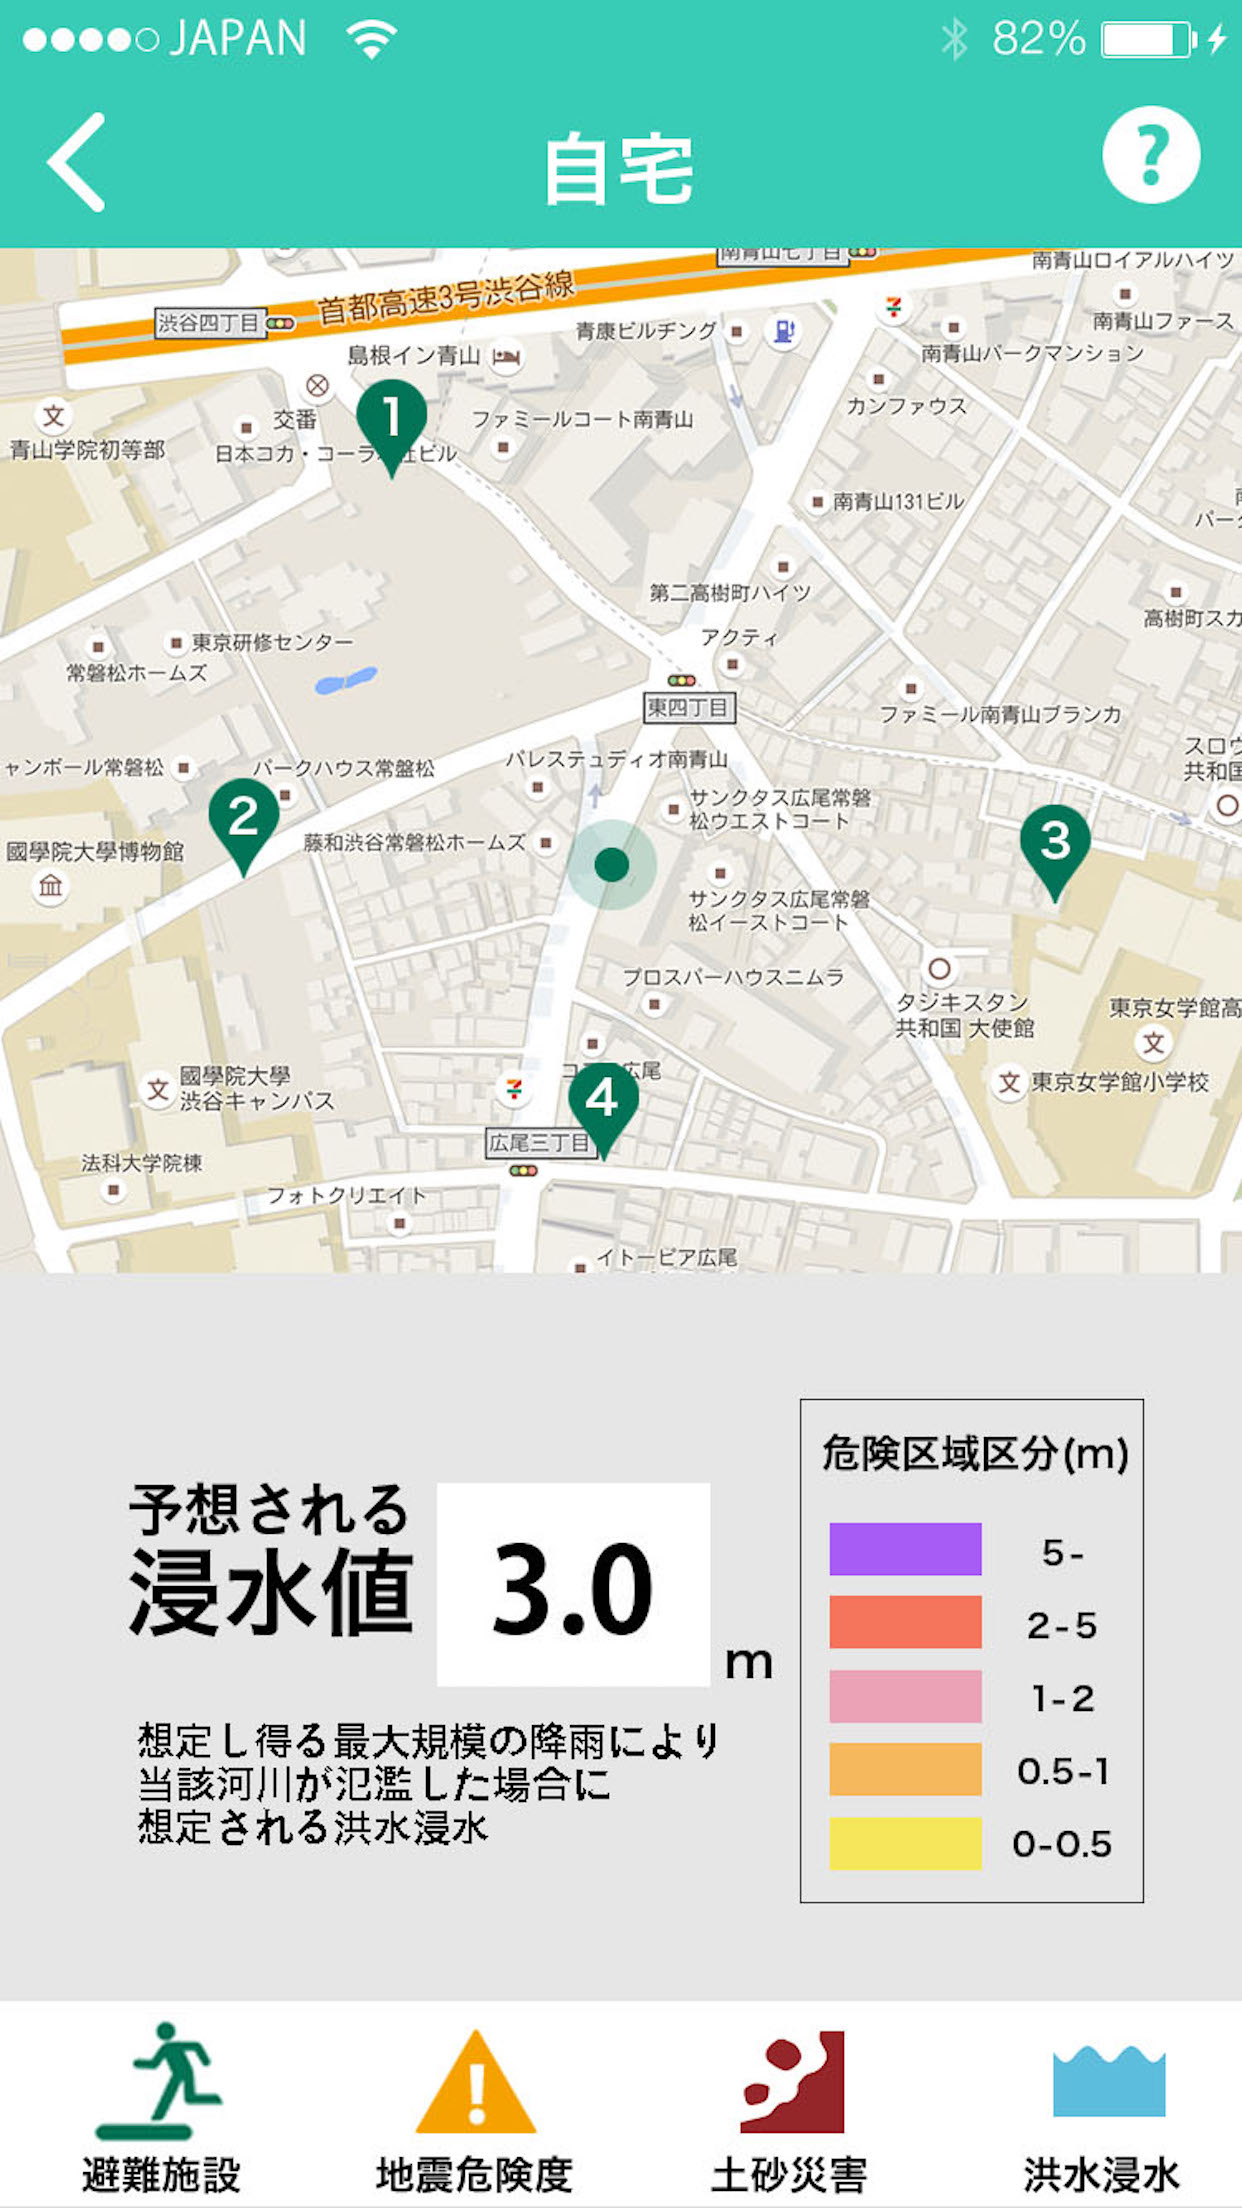
\includegraphics[width=\hsize]{./images/mbs_flood.jpg}
    \end{minipage}
    &
    \begin{minipage}{0.3\hsize}
      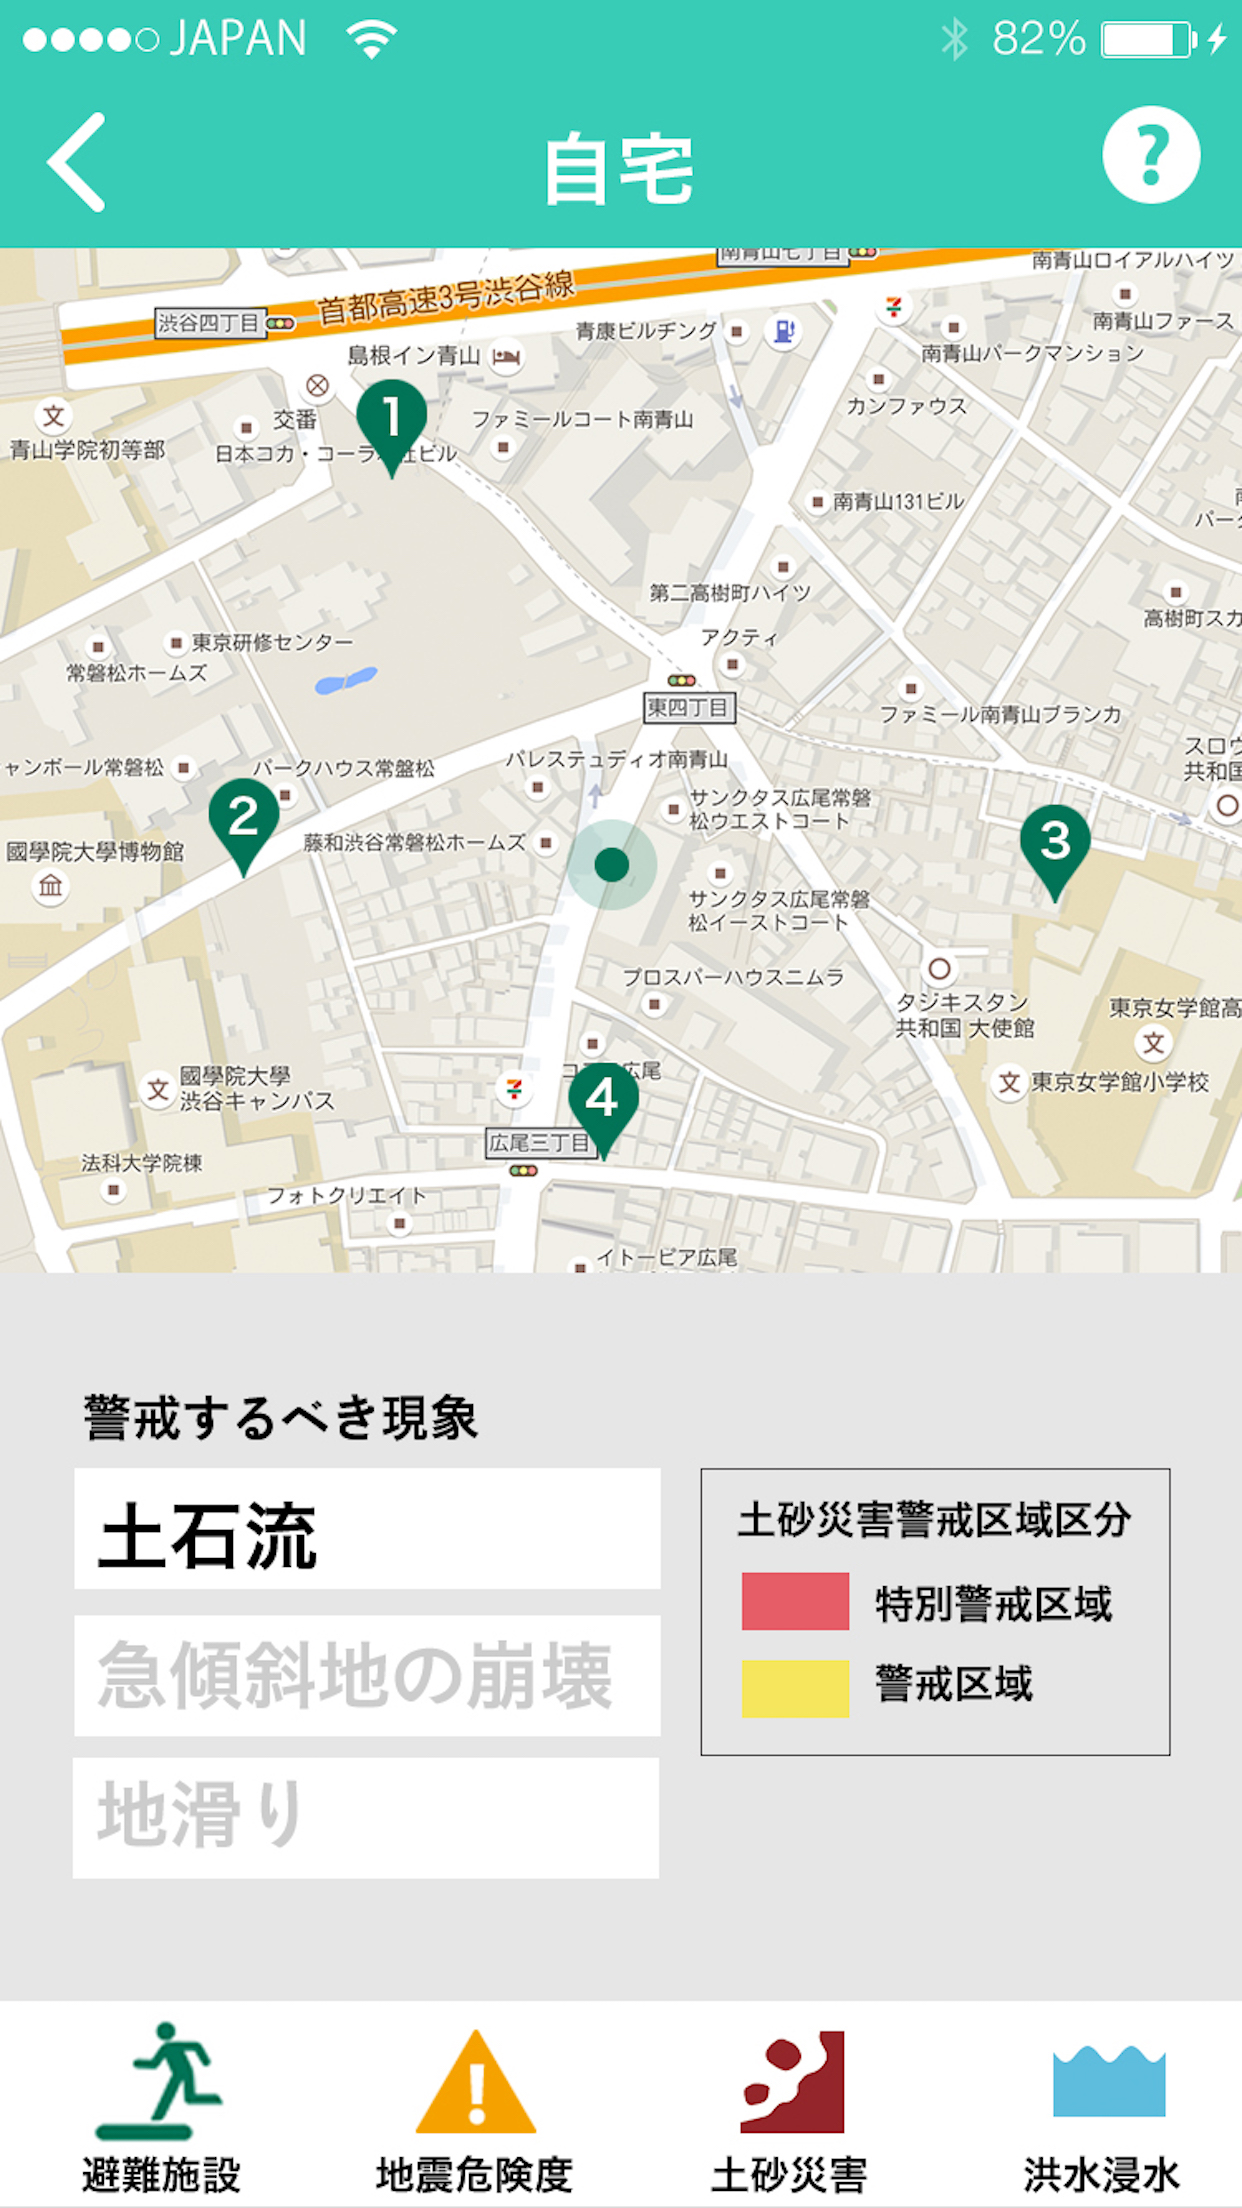
\includegraphics[width=\hsize]{./images/mbs_sediment.jpg}
    \end{minipage}

  \end{tabular}
    \caption{防災情報画面(左:地震危険度,中:洪水浸区域,右:土砂災害警戒区域)}
    \label{fig:screen-structure-02}
  \end{center}
\end{figure}
\fi


\subsection{実証実験}
神奈川県鎌倉市で実施された国土地理院主催の防災アプリの実証実験にて,本アプリの評価検証を行う.
実証実験では参加者によるディスカッションも行われ,その後参加者に対象にアンケート調査を行う.
% 本アプリは実験用のアプリとして使用する.

\subsubsection{実験の概要}
実証実験の概要を表\ref{tab:kamakura-general}に示す.
実証実験は,防災アプリを使用して自然災害に対するリスクを把握し,適切な災害対応への理解を深めることを目的とし,平成27年の国土地理院主催の防災アプリケーションコンテストで優秀アプリとして選定された防災学習アプリ三つが用いられた.本アプリは当コンテストで選定され,筆者は開発者として実証実験に参加した.
実証実験のプログラムは以下のように構成される.

\begin{enumerate}
  \item 参加者による鎌倉市内を使った実証実験

  グループごとに別れて鎌倉市内を歩き,防災アプリを通して自然災害発生時のリスクや適切な対応への理解を深める実験を実施.

  \item 参加者と開発者によるグループディスカッション

  実証実験終了後に,必要と考える防災アプリの機能や,災害対応を考える上で有効な防災情報等について,参加者及び開発者による意見交換を実施.

  \item アンケート調査

  実証実験で使用した防災アプリの機能や操作性についての評価,アプリに求める防災情報等について紙のアンケート調査を実施.

\end{enumerate}

実証実験は1日限りの開催のため,当日アプリをインストールするユーザは生活圏の検出を十分に行えないため,鎌倉市在住と仮定する仮想のユーザデータを入れたアプリを実装し,参加者の端末にインストールして実証実験を行ってもらった.
実証実験では,アプリを通じて周辺の避難施設や災害時のリスクを確認する様子が見られた(図\ref{tab:kamakura-general}左).グループディスカッションでは,防災アプリに関する活発な意見交換が行われ,本アプリへのコメントでは「他の防災アプリは使いづらいものが多いが,シンプルなインタフェースで情報を絞り込まれていてわかりやすい」といった操作性・閲覧性を評価するものや「家族間で情報を共有したい」「オフラインでも使えるようにしたい」といった,機能の追加や向上を求める意見がみられた(図\ref{tab:kamakura-general}右).

\begin{table}[H]
  \begin{center}
    \caption{実証実験の概要}
    \renewcommand\arraystretch{1.4}
    \begin{tabular}{|c|l|}
      \hline
      名称 & 鎌倉市におけるリスクコミュニケーション実証実験 \\
      \hline
      主催 & 国土交通省 国土地理院 \\
      \hline
      日程 & 平成27年11月14日(土) \\
      \hline
      時間 & 9時30分~15時45分 \\
      \hline
      場所 & 神奈川県鎌倉市 \\
      \hline
       参加者  & 約70名 \\
      \hline
    \end{tabular}
    \label{tab:kamakura-general}
  \end{center}
\end{table}

\fifigure
\begin{figure}[H]
  \begin{center}
    \begin{tabular}{cc}
    \begin{minipage}{0.5\hsize}
	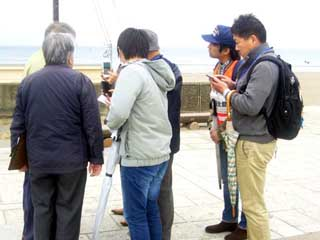
\includegraphics[width=\hsize]{./images/kamakura_01.jpg}
    \end{minipage}
    &
    \begin{minipage}{0.5\hsize}
      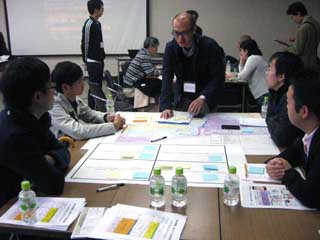
\includegraphics[width=\hsize]{./images/kamakura_02.jpg}
    \end{minipage}
  \end{tabular}
    \caption{左:アプリで避難施設や災害時リスクを確認する様子,右:グループディスカッションの様子}
    \label{fig:kamakura-01}
  \end{center}
\end{figure}
\fi

\subsubsection{評価}
イベントに参加した述べ70名のうち,35名からアンケートの回答を得ることができた.

\begin{enumerate}
  \item アンケート内容

  アンケートの内容は表\ref{tab:kamakura-questionnaire-content}の通りである.

  \begin{table}[H]
    \begin{center}
      \caption{アンケートの内容}
      \renewcommand\arraystretch{1.2}
      \begin{tabular}{|c|l|}
        \hline
        設問1 & \multicolumn{1}{p{10cm}|}{防災アプリの使いやすさについて} \\
        & 1.使いやすい \\
        & 2.やや使いやすい \\
        & 3.やや使いやすい \\
        & 4.やや使いにくい \\
        & 5.使いにくい \\
        \hline
        設問2 & \multicolumn{1}{p{10cm}|}{その理由について} \\
        & (自由記述式) \\
        \hline
      \end{tabular}
      \label{tab:kamakura-questionnaire-content}
    \end{center}
  \end{table}

  アプリのユーザビリティや情報の閲覧性,また本開発で用いたシステムの妥当性を検証するため設問1.2を設ける.

  \item 回答者の属性

  回答者の属性を表\ref{tab:kamakura-userstatus}に示す.

  \begin{table}[H]
    \begin{center}
      \caption{回答者の属性}
      \renewcommand\arraystretch{1.4}
      \begin{tabular}{|c|c|c|c|c|c|c|}
        \hline
        \multicolumn{1}{|c|}{回答者数} & \multicolumn{6}{c|}{35名} \\
        \hline
        性別 & \multicolumn{3}{c|}{男性} & \multicolumn{3}{c|}{女性} \\
        \cline{2-7}
        & \multicolumn{3}{c|}{29名} & \multicolumn{3}{c|}{6名} \\
        \hline
        \multicolumn{1}{|c|}{居住地} & \multicolumn{2}{c|}{鎌倉市内} & \multicolumn{2}{c|}{鎌倉市外} & \multicolumn{2}{c|}{未回答} \\
        \cline{2-7}
        & \multicolumn{2}{c|}{6名} & \multicolumn{2}{c|}{28名} & \multicolumn{2}{c|}{1名} \\
        \hline
        年代 & 20代未満 & 20代 & 30代 & 40代 & 50代 & 60代以降 \\
        \cline{2-7}
        & 8名 & 11名 & 6名 & 5名 & 1名 & 4名 \\
        \hline
        職業 & 公務員 & 会社員・自営業 & 研究者 & 学生 & その他 &  \\
        \cline{2-7}
        & 2名 & 13名 & 1名 & 16名 & 3名 & \\
        \hline
      \end{tabular}
      \label{tab:kamakura-userstatus}
    \end{center}
  \end{table}

  市外からの参加者が多く,男性が29名と偏りはあるものの,職場で防災を担当しているという会社員や高校生・大学生,公務員等,様々な世代,職種の人からの回答が集まった.

  \item 結果

  アンケート結果のグラフを図\ref{fig:kamakura-questionnaire}に,記述回答の内容を表\ref{tab:kamakura-comment}に示す.

  \fifigure
  \begin{figure}[H]
    \begin{center}
      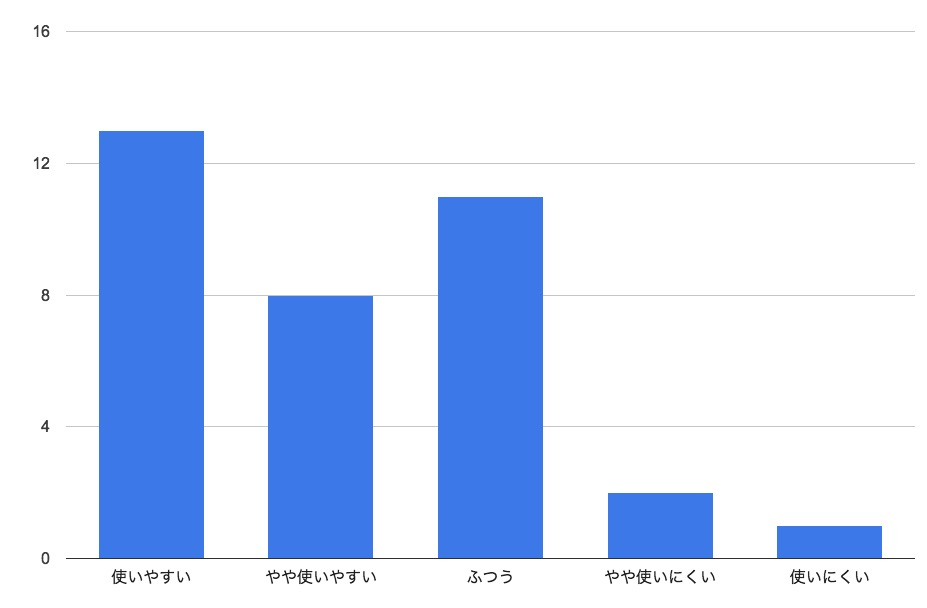
\includegraphics[width=0.8\hsize]{./images/kamakura_questionnaire.jpg}
      \caption{アンケート結果(アプリの使いやすさついて)}
      \label{fig:kamakura-questionnaire}
    \end{center}
  \end{figure}
  \fi

  \begin{table}[H]
    \begin{center}
      \caption{アンケート結果(アプリの使いやすさに関する回答)}
      \renewcommand\arraystretch{1.2}
      \begin{tabular}{|p{15cm}|}
        \hline
        \multicolumn{1}{|c|}{使いやすい・やや使いやすいと答えた人の理由} \\
        \hline
        ・インターフェースが良い。\\
        ・現在地や自分のよくいく場所によって避難所が出てくるのは良かったから。\\
        % ・日常面での使用に将来性があるように思った。 \\
        ・機能や内容がシンプルにまとめてあって使いやすかったです。\\
        ・自宅以外での防災拠点がわかるのは良い。
        % バックグラウンドで動くようなので、電池の消費が災害時にもったいない。\\
        ・まだ活用できるだけの情報がたまっていないが、情報が増えるなど使いやすくなりそうだ。\\
        % ・普段自分の生活圏内での情報をしっかり記録してくれる機能があるのがよかった。\\
        ・自分に必要な情報だけ出るから。\\
        ・とても見やすかった。普段使う場所の情報が厳選表示されるのは良いと思う。\\
        ・身のまわりの情報が出てくるのがありがたい。少し情報は少なめだが、わかりやすいと思った。\\
        % ・シンプルで良い。\\
        \hline
        \multicolumn{1}{|c|}{使いにくい・やや使いにくいと答えた人の理由} \\
        \hline
        % ・Googleビューが、災害時の状況を反映させたものか疑問 \\
        ・良く落ちる。動作不安定。しかし今後に期待する。 \\
        ・インストールから使用まで、手間を要する。 \\
        \hline
      \end{tabular}
      \label{tab:kamakura-comment}
    \end{center}
  \end{table}

  「アプリの使いやすさいについて」の設問では,60\%が「使いやすい」と回答した(「使いやすい」13名+「やや使いやすい」8名).使いやすかった理由として「インターフェースが良い」「機能や内容がシンプルにまとめてあって使いやすかったです。」といった,アプリのインタフェースデザインを評価する回答や「普段使う場所の情報が厳選表示されるのは良いと思う。」「自宅以外での防災拠点がわかるのは良い。」といった,生活圏に合わせて絞り込まれた情報を評価する回答がみられた.
  反対に「使いにくい」と回答した人は8\%いた(「やや使いにくい」2名+「使いにくい」1名).その理由として「良く落ちる。動作不安定。」というシステム面を指摘する回答や,「インストールから使用まで、手間を要する。」という,生活圏の検出までの期間を指摘する回答が見られた.
\end{itemize}


\subsection{アプリ公開後の評価}
前節で述べた実証実験でのアンケート調査に加え,開発したアプリをWeb上で公開し,実際に生活圏が検出されたと思われるユーザを対象にWEBアンケートを実施した.
アプリは,iOS向けアプリ配信サービスのApp Storeで配信を行い,アプリ内にWEBアンケートへのリンクを設置した.

  \begin{enumerate}
    \item アンケートの内容

    アンケートの項目は実証実験と同様に,アプリの使いやすさとその理由についての設問を設置し,加えてその他アプリに対する意見として自由記述の設問を設けた.

    \item 回答者の属性

    回答者の属性を表\ref{tab:mbn-userstatus}に示す.


    \begin{table}[H]
      \begin{center}
        \caption{回答者の属性}
        \renewcommand\arraystretch{1.4}
        \begin{tabular}{|c|c|c|c|c|c|c|}
          \hline
          \multicolumn{1}{|l|}{回答者数} & \multicolumn{6}{c|}{17名} \\
          \hline
          性別 & \multicolumn{3}{c|}{男性} & \multicolumn{3}{c|}{女性} \\
          \cline{2-7}
          & \multicolumn{3}{c|}{16名} & \multicolumn{3}{c|}{1名} \\
          \hline
          年代 & 20代未満 & 20代 & 30代 & 40代 & 50代 & 60代以降 \\
          \cline{2-7}
          & 0名 & 8名 & 2名 & 5名 & 1名 & 1名 \\
          \hline
          職業 & 公務員 & 会社員・自営業 & 研究者 & 学生 & その他 &  \\
          \cline{2-7}
          & 1名 & 5名 & 0名 & 5名 & 6名 & \\
          \hline
        \end{tabular}
        \label{tab:mbn-userstatus}
      \end{center}
    \end{table}

    Webアンケートでは述べ17名の回答を得た.男性が16名と偏りはあるものの,世代・職種ともに様々な属性の人からの回答が集まった.

    \item 結果

    アンケート結果のグラフを図\ref{fig:mbn-questionnaire}に示す.またその理由についての記述回答と,その他アプリに対する意見の内容を表\ref{tab:mbn-comment}に示す.


    \fifigure
    \begin{figure}[H]
      \begin{center}
        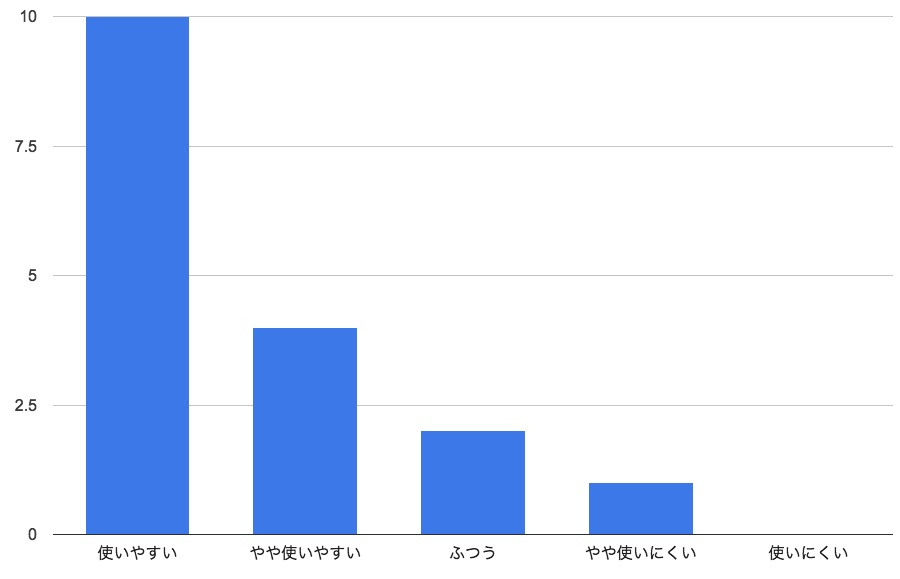
\includegraphics[width=0.8\hsize]{./images/mbn_questionnaire.jpg}
        \caption{アンケート結果(アプリの使いやすさついて)}
        \label{fig:mbn-questionnaire}
      \end{center}
    \end{figure}
    \fi

    \begin{table}[H]
      \begin{center}
        \caption{アンケート結果(アプリの使いやすさに関する回答)}
        \renewcommand\arraystretch{1.2}
        \begin{tabular}{|p{15cm}|}
          \hline
          \multicolumn{1}{|c|}{使いやすい・やや使いやすいと答えた人の理由} \\
          \hline
          % ・わかりやすい。\\
          % ・一目でわかるから\\
          ・自分の家の近くの避難場所がすぐ分かる。 \\
          ・身近な地域での防災について学習する機会があまりなく、アプリがよいきっかけになった \\
          ・平時に訪れた場所や町がどの程度の災害に遭うのかを予備知識として知っておくのは有用。\\
          ・自分のいる場所の情報がわかりやすい\\
          ・はじめての土地の避難場所検索や災害の脆弱性を知るのに便利だった\\
          ・感覚で操作できる。\\
          ・インターフェースがシンプルで良い\\
          % ・デザインが良い\\
          % ・見やすい\\
          % ・いる場所の避難場所がすぐ分かる。
          \hline
          \hline
          \multicolumn{1}{|c|}{使いにくい・やや使いにくいと答えた人の理由} \\
          \hline
          ・使うタイミングが分からない。\\
          \hline
          \hline
          \multicolumn{1}{|c|}{その他アプリに対する意見} \\
          \hline
          ・このアプリを使うことで利用者がそのように防災の取り組みをしていけばいいかについて、ガイドがない \\
          % ・アプリを起動していなくても位置情報は送信されるの?
          ・プレビューと地図が一致していない。\\
          ・地震の確率より、それぞれの地域の揺れやすさ等が分かると良い \\
          ・地震情報だけ数値ででていて、その数字で災害の危険性に対する実感がわかない。\\
          ・場所によっては、「洪水浸水」の予想される浸水地で表示される数字が判例の色と異なっている。\\
          \hline
        \end{tabular}
        \label{tab:mbn-comment}
      \end{center}
    \end{table}

    使いやすかった理由として「インターフェースが良い」「機能や内容がシンプルにまとめてあって使いやすかったです。」といった,アプリのインタフェースデザインを評価する回答や「普段使う場所の情報が厳選表示されるのは良いと思う。」「自宅以外での防災拠点がわかるのは良い。」といった,生活圏に合わせて絞り込まれた情報を評価する回答がみられた.
    「アプリの使いやすさいについて」の設問では,82\%が「使いやすい」と回答した(「使いやすい」10名+「やや使いやすい」4名).
    使いやすかった理由として,実証実験と同じくインタフェースデザインを評価する回答が多くみられた他,
    「自分のいる場所の情報がわかりやすい」「はじめての土地の避難場所検索や災害の脆弱性を知るのに便利だった」といった,ユーザの現在地に合わせた情報提示を評価する意見がいくつかみられた.
    「やや使いにくい」と回答した人は1名で,「使いにくい」と回答した人は一人もいなかった.
    しかし「やや使いにくい」と回答した人の「使うタイミングが分からない。」という記述や,自由意見での「このアプリを使うことで利用者がそのように防災の取り組みをしていけばいいかについて、ガイドがない」といった,アプリの利用方法やタイミングに迷ってしまう意見がみられた.
    また,その他の自由意見では,地震危険度や洪水浸水想定区域の表記や精度を指摘する回答が多くみられた.

  \end{itemize}
% 実証実験では仮想のユーザデータを入れたアプリを用いた評価を行ったので〜



\subsection{考察}
実証実験及びアプリ公開後でそれぞれ実施したアンケート調査の結果を元に,生活圏に基づいて情報の絞り込みを行う本アプリの利用可能性について考察する.

実証実験とアプリ公開後で共通して,過半数のユーザが本アプリを「使いやすい」と回答し,絞り込まれた情報の見やすさやインターフェースデザインの評価がその理由にあげられた.
これは,本アプリで用いたシステム及びインタフェースが,ハザードマップの情報の閲覧性やアプリのユーザビリティを向上させる要因になったといえる.
公開後の回答でアプリの利用方法やタイミングに迷ってしまう意見がみられたが,これは,実証実験と違い,日常ではアプリを使用する目的が明確に示されていないためであると考えられる.
また実証実験では,普段から防災アプリを使用する人が多く集まったことから,ディスカッションでは他のアプリと比較する議論が起こり,その中で本アプリの操作性や閲覧性を評価する意見が見られた.

このことから,検出された生活圏に基づき,ハザードマップの情報を絞り込んでユーザに提示する本手法により,既存のハザードマップアプリの操作性や閲覧性の低さを解決できたといえる。一方,防災情報の表記や精度への指摘が目立ったことを踏まえ,データの精度やインタフェースの工夫を検討することが今後の課題であるといえる.

% 全体を通して,生活圏だけでなく,ユーザの現在地に合わせた情報提示を評価する意見がいくつかみられた
% 生活圏の割り出しまでの期間を指摘する回答が見られたが

% 場合によっては,二章で紹介したwatav\cite{}や
% のような,ユーザ選択型の適応も考えられる?


\section{キュレーションアプリにおけるパーソナライズ}
本章では,三章で開発したフレームワークを組み込み,検出された生活圏をもとにWebメディアの情報を絞り込んでユーザに提示するキュレーションアプリの仕様と実装について述べる.さらにアプリ公開後に実施したアンケート調査の結果と考察について述べる.


\subsection{キュレーションアプリの概要と開発の目的}
特定のテーマに沿って複数のサイトの情報を収集・編集し提示するメディアをキュレーションメディアと呼び,キュレーションアプリはそれをスマートフォンアプリとして利用できるようにしたものである.
近年,インターネット上で日々大量のメディアコンテンツが生産される中,サービス側が情報収集を行うキュレーションサービスは注目を集めている\cite{ohmukai}.
事例として
「SmartNews\footnote{https://www.smartnews.com/ja/}」「Antenna\footnote{https://antenna.jp/}」「watav\footnote{http://watav.com/}」などがあり,これらは二次メディアとして他のメディアから記事のデータを収集し,概要をサイトやアプリ内でまとめ,個々の記事への導線を作っている.
記事の選別は,独自のアルゴリズムを元にプログラムによって行う場合もあれば,人の手によって行う場合もある.

一方,近年生まれたサービス形態であることからキュレーションメディアの定義は曖昧であり,
キュレーターと呼ばれる人がインターネット上の情報を収集し記事にまとめたものを置く形態や,
一般のユーザが自由にまとめ記事を作成し共有する形態を指す場合もある.
本研究においてキュレーションメディアは,前述した事例に合わせ「特定のテーマに沿って複数のメディアからデータを収集し,記事への導線と概要をまとめた二次メディア」と定義する.

こういったキュレーションメディアを扱うスマートフォンアプリは,パーソナライズの事例が既に多く見られる分野である.
「watav」は,二章の先行事例で述べたように,登録したユーザの属性や過去の閲覧履歴を元にユーザの趣味嗜好に合わせたイベント情報を絞り込んで提示している.
しかし,蓄積した位置情報を用いて情報の選定を行う事例は見られない.
そこで,既にパーソナライズの事例が多く見られる分野において新たな手法を創出することを目的とし,検出された生活圏に基づいてWebメディアの情報を絞り込んで提示するキュレーションアプリを開発する.
% インターネット上に散在するWebメディアの情報を,ユーザの生活圏に基づいて収集し提示することで,

% Webメディアの中から,ユーザの周囲に溢れる情報を集めることが可能,新たな切り口を創出することが可能だと予想する.
% 本開発の目的は,既にパーソナライズの事例が多く見られるキュレーションサービスの分野で,ユーザの生活圏に基づいて絞り込みを行う,という新たな手法を創出し,その利用可能性を示すことである.

\subsection{利用データの設計}
開発するアプリで利用するWebメディアのデータ設計及びAPIの仕様について述べる.
絞り込みの対象となるデータは実空間の情報に紐づけられるものが望ましいことから,
グルメ,観光・イベント,エンターテイメントなど,特定の店舗や施設に関連するジャンルの情報(以降,スポット情報と表記)
を扱い,記事内部に一定のフォーマットを持ち,施設や場所の住所が抽出可能なメディアを本アプリにおける一次メディアとして選定する.

% アプリケーションからWebメディアの情報を位置情報に基づいて取得可能にするため,
% 次いで,各メディアのサイトを対象にウェブスクレイピングを行い,位置情報を付加したデータをオリジナルのデータベースに追加次いでAPIを実装する.

記事の概要がリスト化されたページのウェブスクレイピングを行い,
サムネイル画像,詳細ページのURL,記事の作成日時,記事タイトルなどの情報を取得する(図\ref{fig:curation-scraping-list}).
取得したURLから記事ページのHTMLデータを取得し,正規表現を用いて記載された箇所から住所を抽出する(図\ref{fig:curation-scraping-article}).
ジオコーディングAPIを用いて,緯度経度,都道府県名,地域名をそれぞれ取得し,ウェブスクレイピングで得た情報と併せてデータベースに格納する.
その結果,データベースのカラムは表\ref{tab:curation-database}のように定義される.
このデータベースから,緯度経度のリストを含んだリクエストを投げることで,各地点において一定範囲内に存在する記事データのレスポンスが帰ってくるAPIを実装し,これを本アプリの開発に組み込む.
% (記事取得APIの詳細書く?)

\fifigure
\begin{figure}[H]
  \begin{center}
    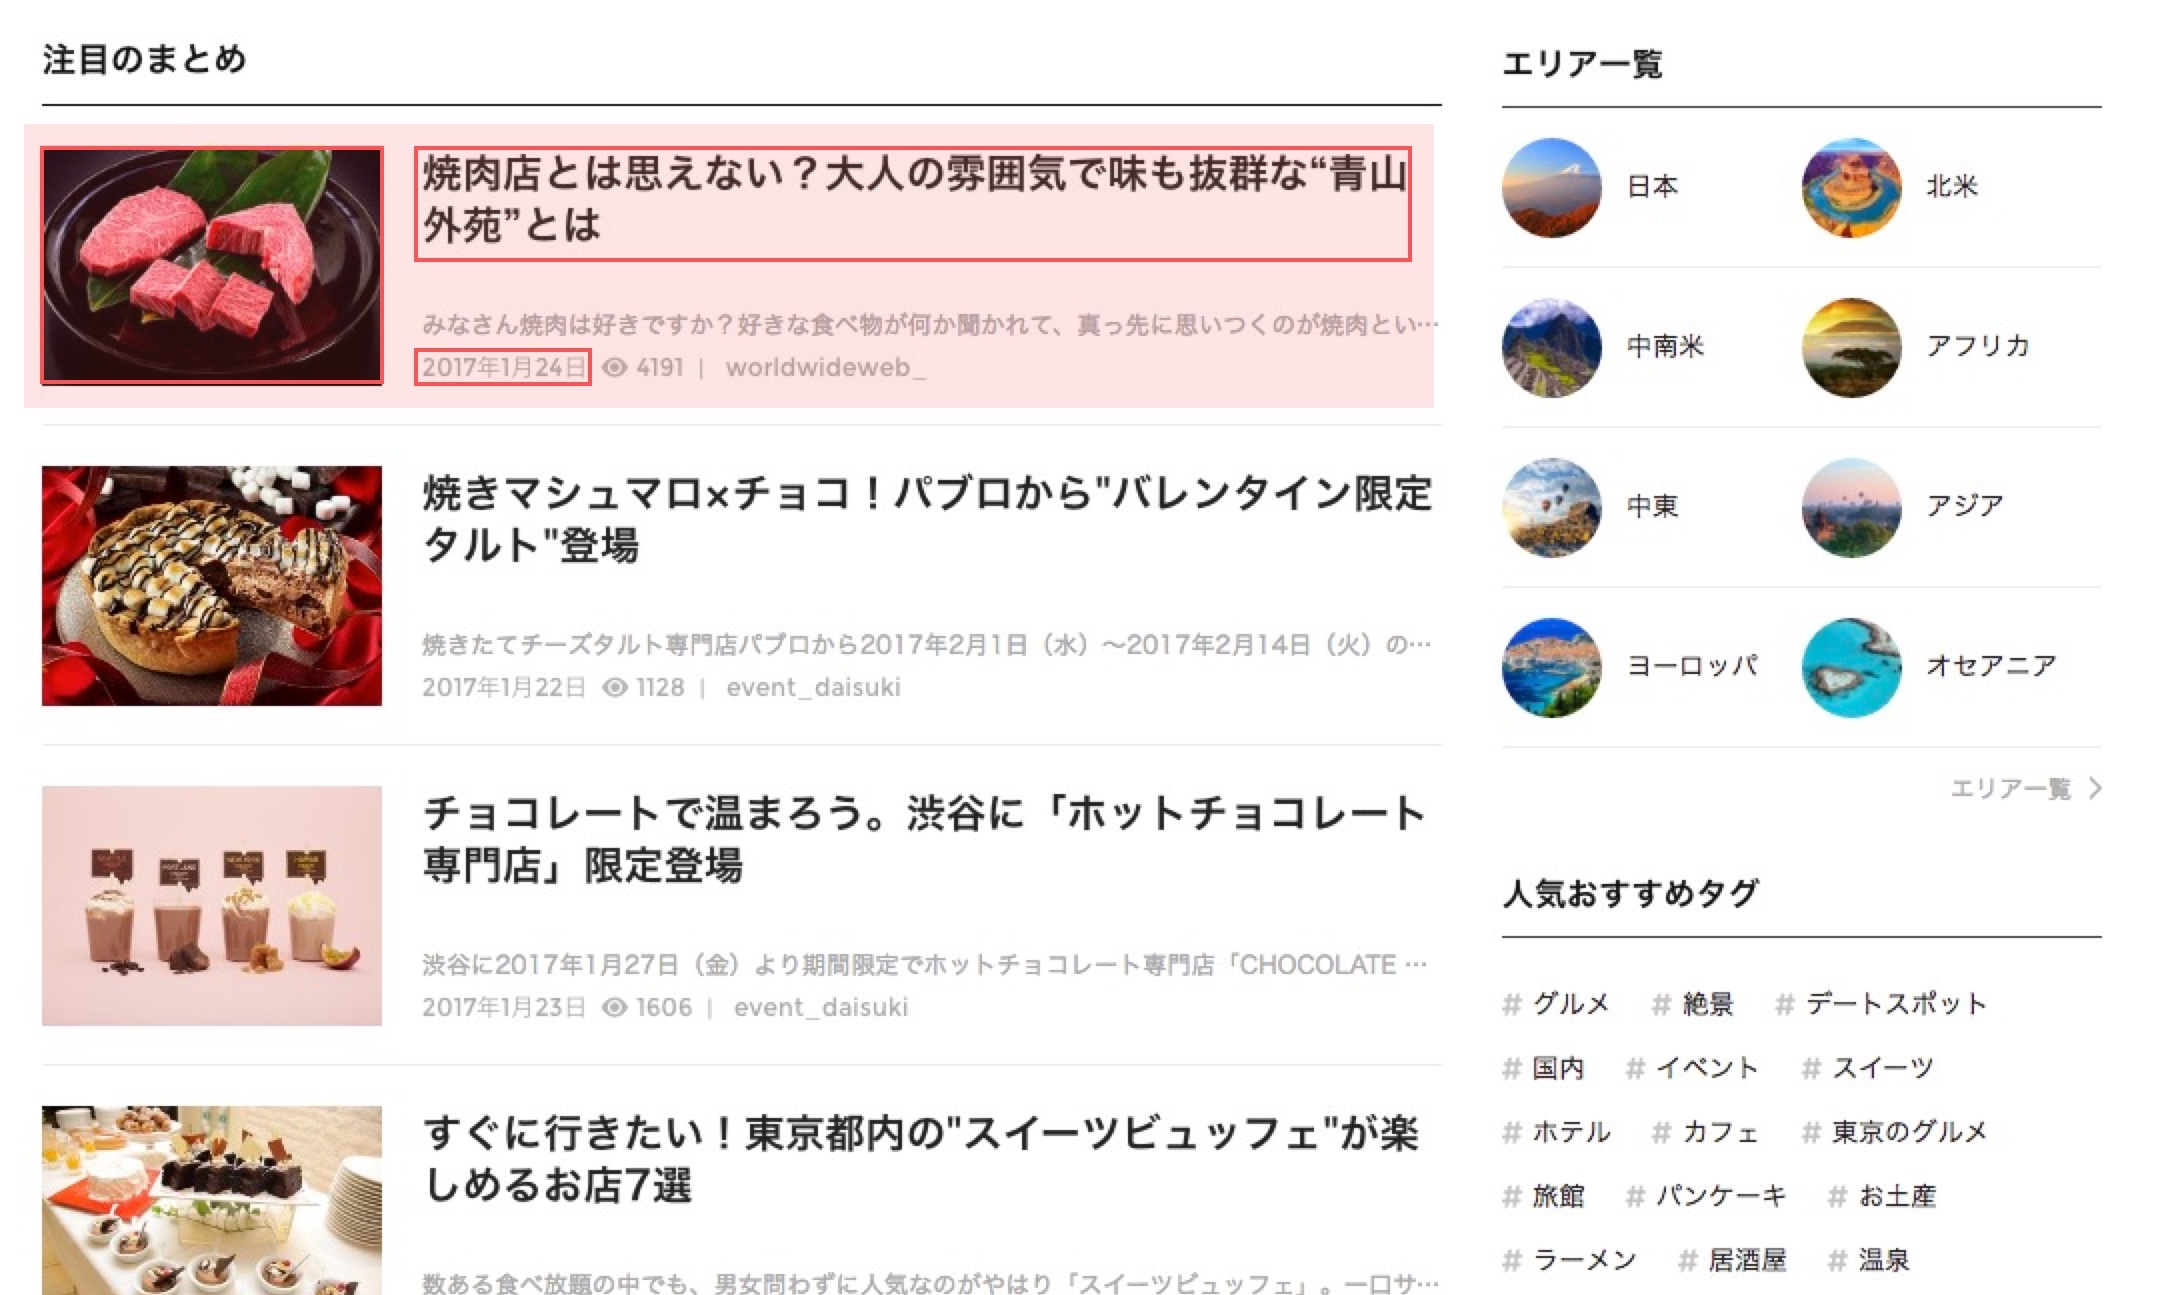
\includegraphics[width=0.95\hsize]{./images/curation_scraping_list.jpg}
    \caption{記事情報のウェブスクレイピング}
    \label{fig:curation-scraping-list}
  \end{center}
\end{figure}
\fi

\fifigure
\begin{figure}[H]
  \begin{center}
    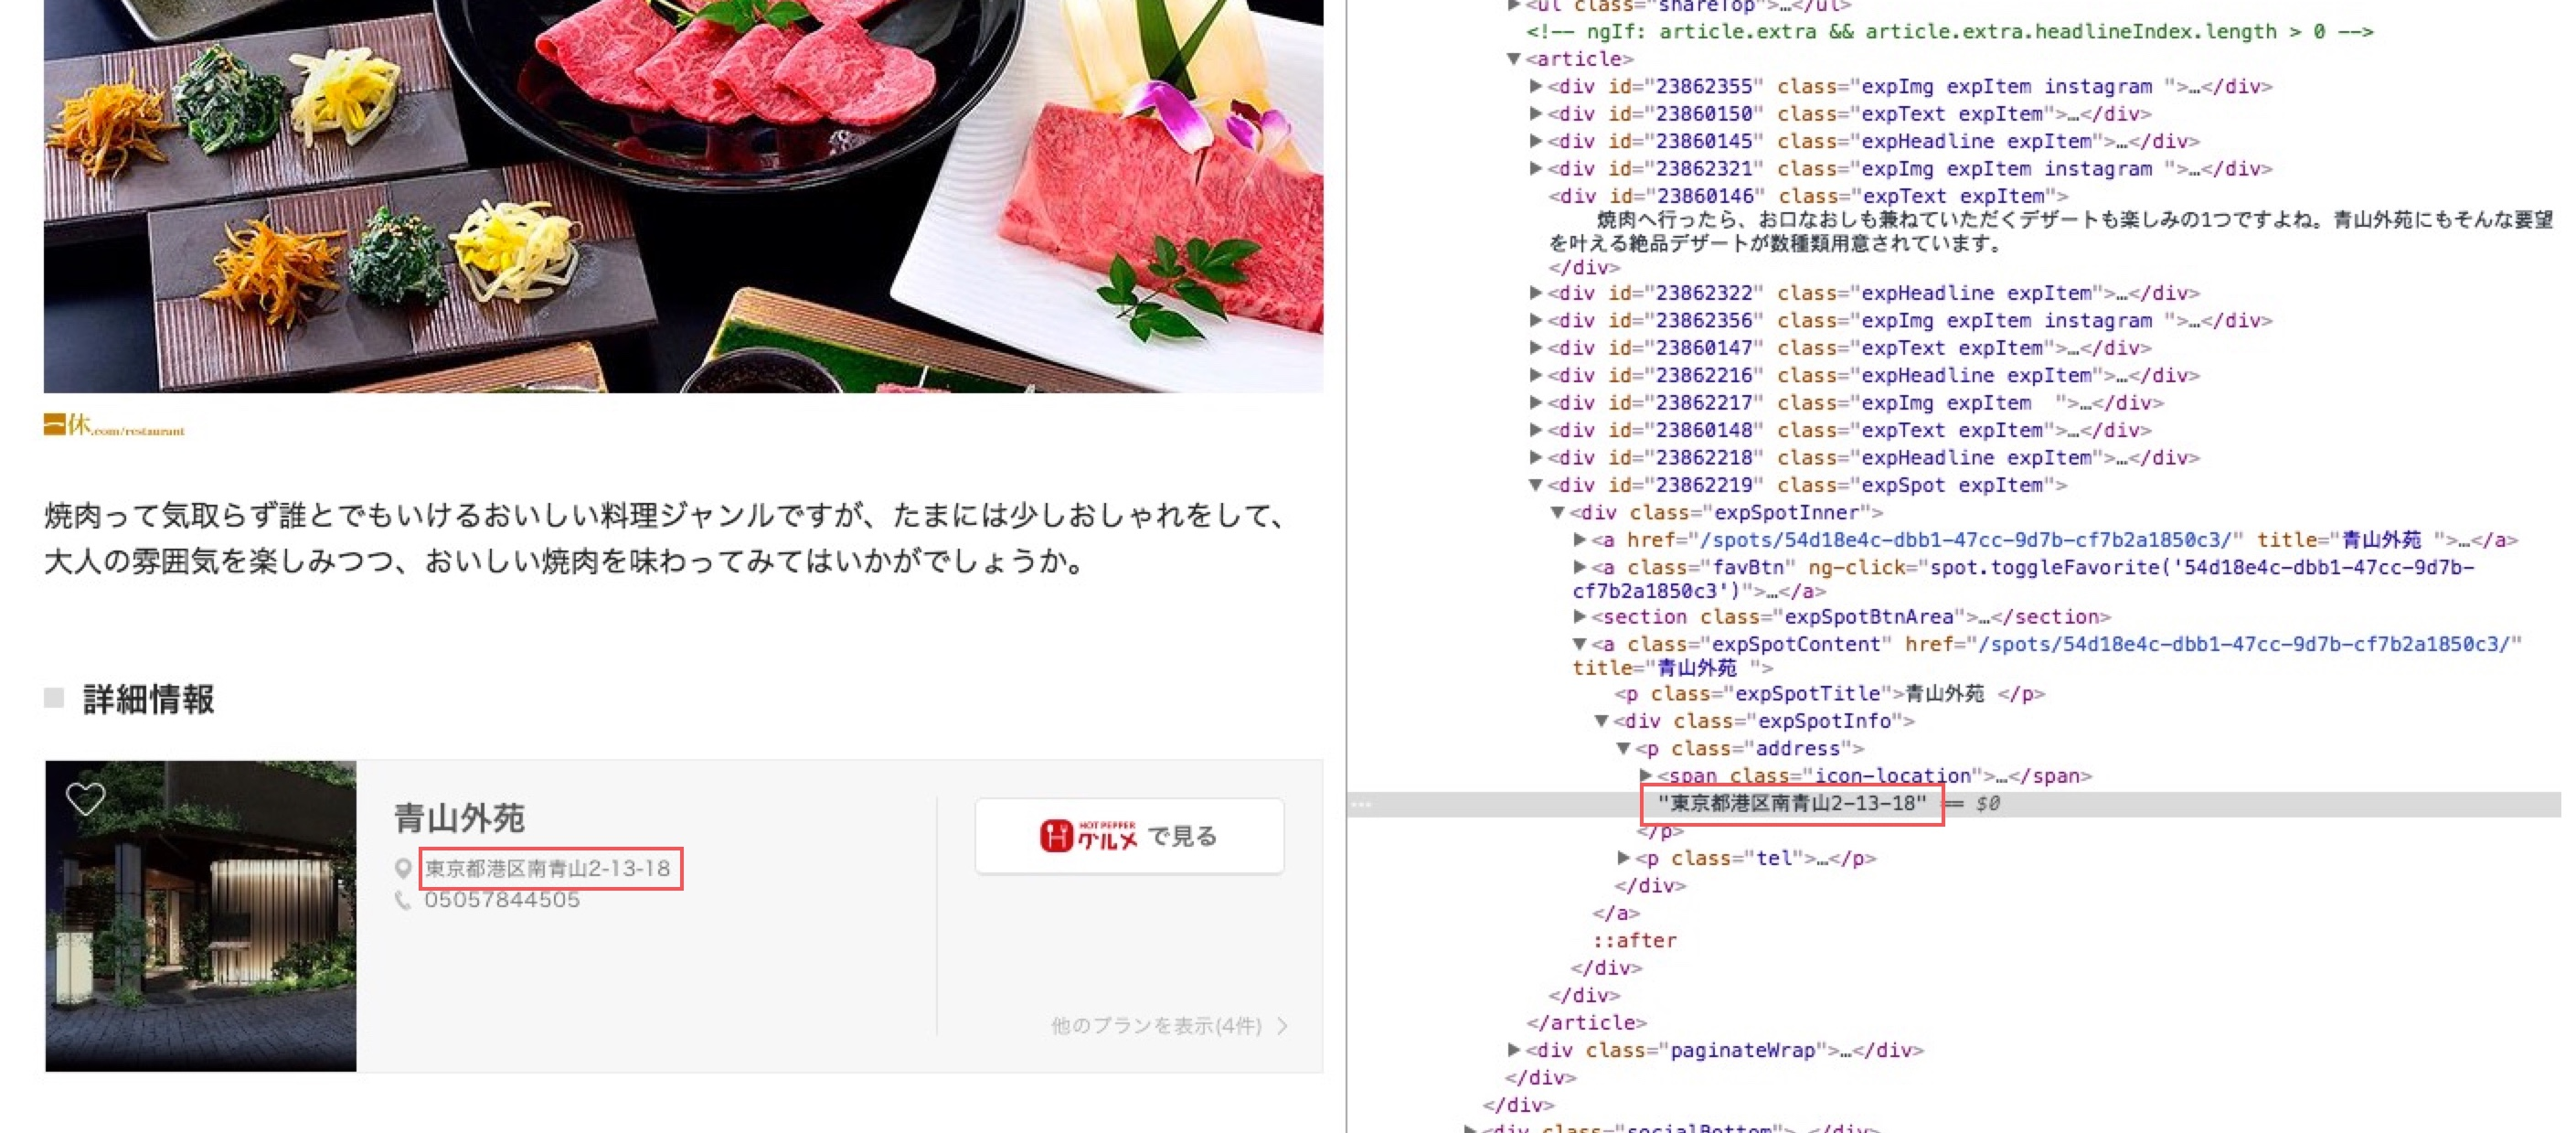
\includegraphics[width=0.95\hsize]{./images/curation_scraping_article.jpg}
    \caption{住所情報の取得}
    \label{fig:curation-scraping-article}
  \end{center}
\end{figure}
\fi

\begin{table}[H]
  \begin{center}
    \caption{メディア情報を持つデータベースのデータセット}
    \renewcommand\arraystretch{1.4}
    \begin{tabular}{|c|c|}
      \hline
      属性情報 & データ型 \\
      \hline
      \hline
      ID & Int \\
      \hline
      記事の位置 &  Geometry(点型)  \\
      \hline
      都道府県名 & String \\
      \hline
      地域名 & String \\
      \hline
      下位地域名 & String \\
      \hline
      記事タイトル & String \\
      \hline
       サムネイル画像URL  & String \\
      \hline
      記事リンクURL & String \\
      \hline
      メディアの名称 & String \\
      \hline
      記事作成・更新日時 & Date \\
      \hline
    \end{tabular}
    \label{tab:curation-database}
  \end{center}
\end{table}


\subsection{画面構成・システム構成}
本アプリは,記事の概要の一覧が見れるフィード画面(図\ref{fig:curation_screen_structure_01}左)を起動時の画面とし,
項目を選択した後,記事ページ画面(図\ref{fig:curation_screen_structure_01}右)へ遷移する.また,フィード画面,記事ページ画面から
お気に入りに登録した記事を閲覧できる画面(図\ref{fig:curation_screen_structure_02}左),現在地及び生活圏のリストから記事を検索できる画面(図\ref{fig:curation_screen_structure_02}右)をタブの選択で切り替えられる画面構成とする.
% また,記事の概要を選択した後,対象のWebページを埋め込んだ画面へ遷移する.
以下,主要画面であるフィード画面と記事ページ画面の仕様について述べる.

\begin{enumerate}
  \item フィード画面

  Webにおけるフィードとは,コンテンツの概要を配信用に一定の形式でまとめた情報のことをいう.
  キュレーションやニュースサイトにおけるフィードでは,個々のページのタイトルや更新日,サムネイル画像,執筆者もしくはメディア名,本文の要約などを含めるのが一般的である.本アプリのフィードでは,一般的な情報に地名の情報を併せて載せることで,自身の生活圏に紐づいた記事であることをユーザに印象付ける.
  画面起動時に,端末内のデータベースからユーザの生活圏データを取得し,前節で述べたAPIを用いて取得した記事データをフィードに一覧表示する.
  記事データは,指定した複数の地点において一定範囲内に含まれる記事の中から,最新の記事かつ指定した地点からの距離が短い記事が優先的に選定される.
  これによりユーザは,Webメディアの情報の中から,自身の生活圏に基づいて絞り込まれた記事の情報を優先的に受け取ることができる.項目を選択した後,記事ページの画面へ遷移する.

  \item 記事ページ画面

  一般的なキュレーションアプリのUIを参考にし,
  ヘッダに記事のタイトル,画面中央部に記事ページを埋め込んだインターフェースにする.
  画面右下のボタンから,記事が指す地点の位置を地図上で確認することができる.また関心のある記事はお気に入りとして保存し,別画面で振り返ることができる.

  % \item お気に入り画面
  %
  % 記事ページ画面で登録した記事がリスト・マップでまとめられ,記事ページ画面へ戦意
  %
  % \item 検索画面
  %
  % 現在地
  %
  % 検索結果

\end{enumerate}

% またこの他,チュートリアル画面で
% 位置情報の取得と,その旨を伝えた




\fifigure
\begin{figure}[H]
  \begin{center}
    \begin{tabular}{cc}
    \begin{minipage}{0.35\hsize}
	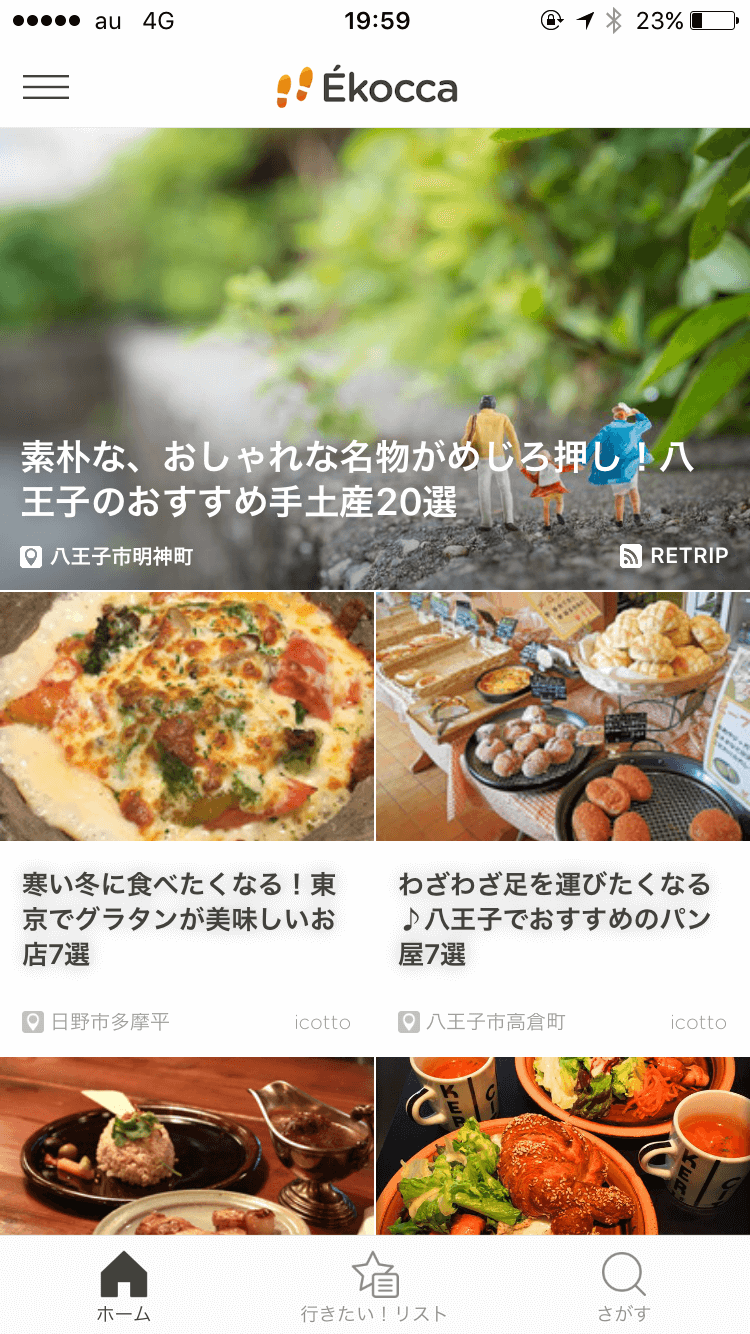
\includegraphics[width=\hsize]{./images/curation_home.png}
    \end{minipage}
    &
    \begin{minipage}{0.35\hsize}
      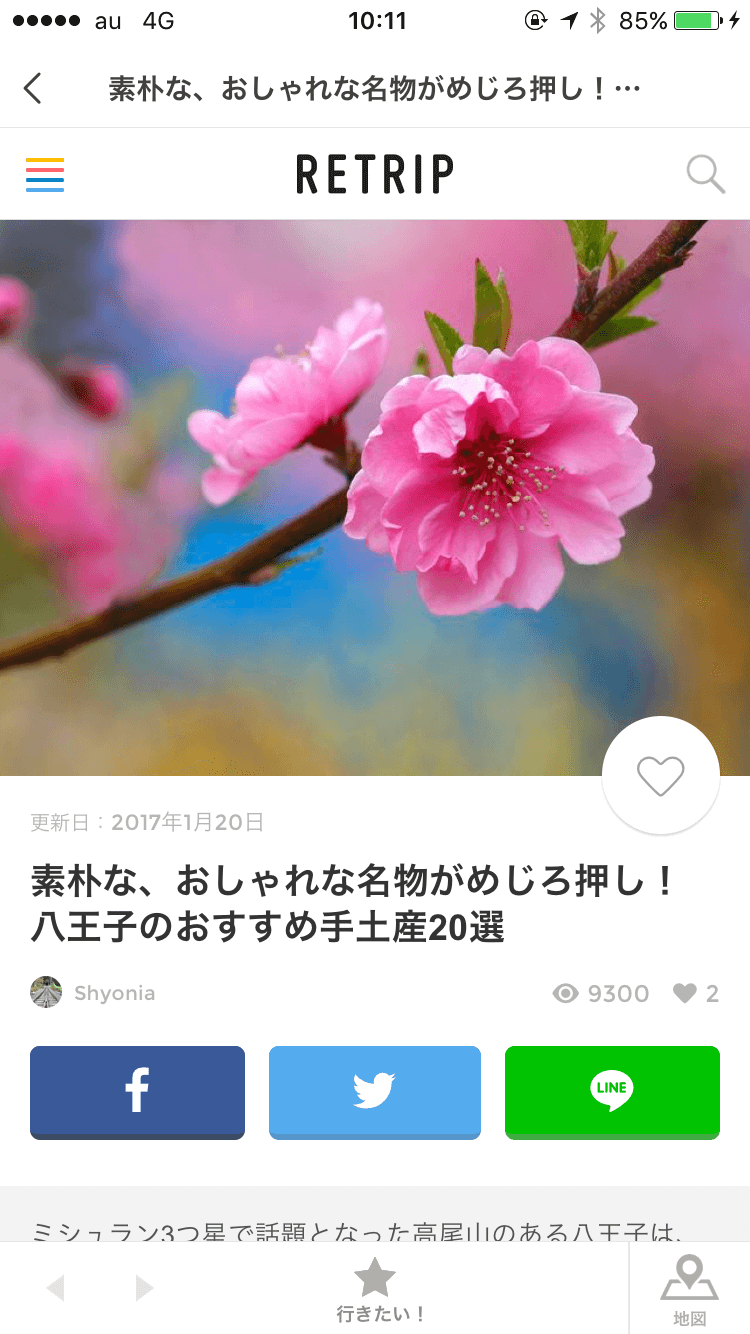
\includegraphics[width=\hsize]{./images/curation_article.png}
    \end{minipage}
  \end{tabular}
    \caption{左:フィード画面,右:記事ページ画面}
    \label{fig:curation_screen_structure_01}
  \end{center}
\end{figure}
\fi

\fifigure
\begin{figure}[H]
  \begin{center}
    \begin{tabular}{cc}
    \begin{minipage}{0.35\hsize}
	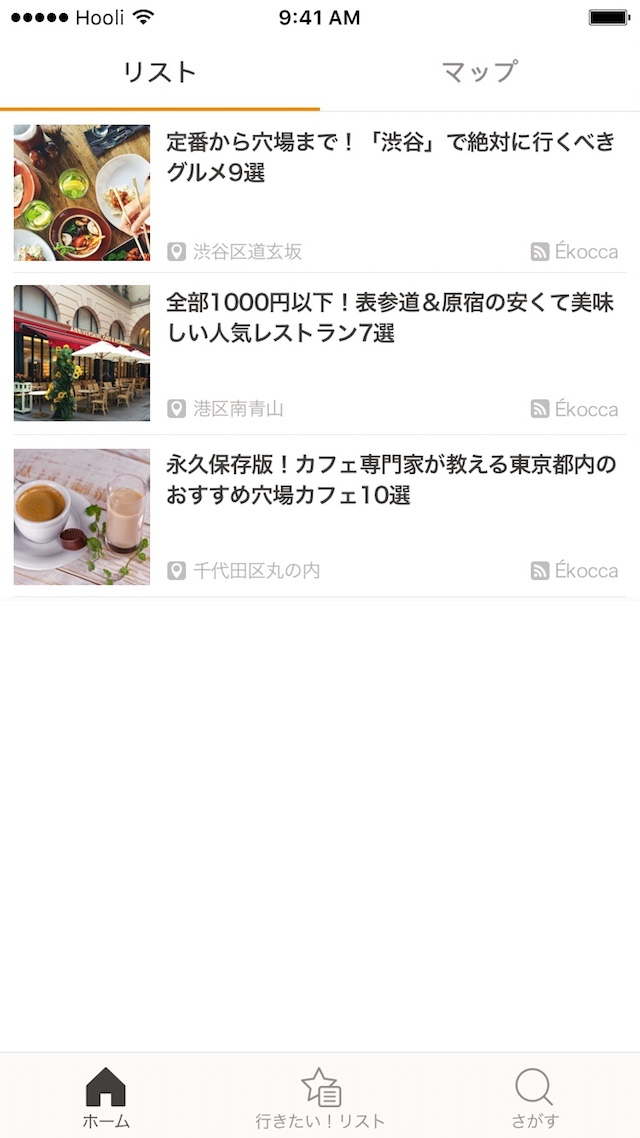
\includegraphics[width=\hsize]{./images/curation_favo_list.jpg}
    \end{minipage}
    &
    \begin{minipage}{0.35\hsize}
      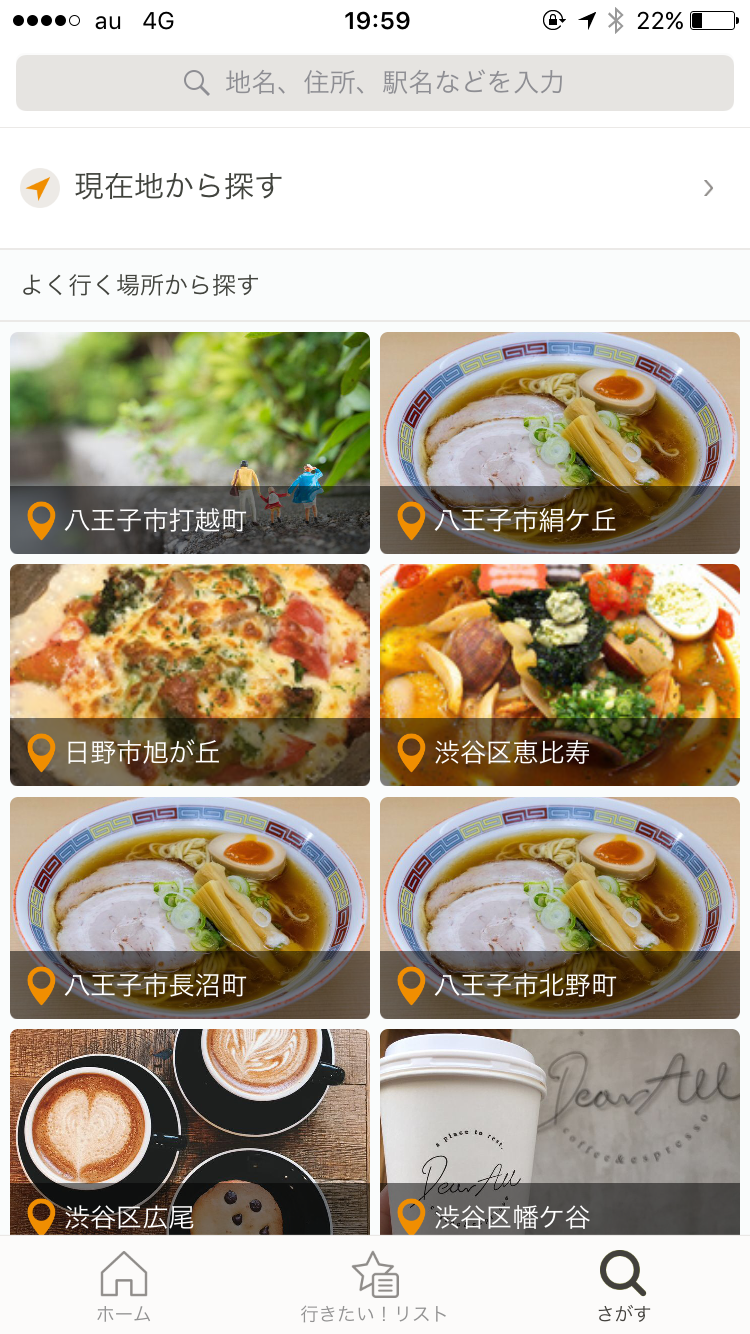
\includegraphics[width=\hsize]{./images/curation_search.png}
    \end{minipage}
  \end{tabular}
    \caption{左:お気に入り画面,右:検索画面}
    \label{fig:curation_screen_structure_02}
  \end{center}
\end{figure}
\fi


\subsection{アプリ公開後の評価}
開発したキュレーションアプリをWeb上で公開し,実際にアプリを使用したユーザを対象にWEBアンケートを実施した.
iOS向けアプリ配信サービスのApp Storeで配信を行い,アプリ内にWEBアンケートへのリンクを設置した.

\begin{enumerate}
  \item アンケート内容

  アンケートの内容は表\ref{tab:curation-questionnaire-content}の通りである.

  \begin{table}[H]
    \begin{center}
      \caption{アンケートの内容}
      \renewcommand\arraystretch{1.4}
      \begin{tabular}{|l|l|}
        \hline
        設問1 & \multicolumn{1}{p{10cm}|}{このアプリを通じて、知ってよかった、行きたいと思った場所の情報はありますか。どのような内容かお答えください} \\
        & (自由記述式) \\
        \hline
        設問2 & \multicolumn{1}{p{10cm}|}{その場所は普段のあなたの生活でどういった場所にあたりますか(選択式)} \\
        & 1.自宅付近 \\
        & 2.学校・勤務先周辺 \\
        & 3.通勤通学の道のり \\
        & 4.その他 \\
        \hline
        設問3 & \multicolumn{1}{p{10cm}|}{アプリで得た情報は役に立ちましたか(選択式)} \\
        & 1.役に立った \\
        & 2.少し役に立った \\
        & 3.ふつう \\
        & 4.あまり役に立たなかった \\
        & 5.役に立たなかった \\
        \hline
        設問4& \multicolumn{1}{p{10cm}|}{その理由について(可能な限り具体的にお答えください)} \\
        & (自由記述式) \\
        \hline
        設問5 & \multicolumn{1}{p{10cm}|}{その他アプリに対するご検討ございましたらご記入ください} \\
        & (自由記述式) \\
        \hline
      \end{tabular}
      \label{tab:curation-questionnaire-content}
    \end{center}
  \end{table}

  本アプリで用いた手法により,ユーザが興味関心を持つ情報を得られたかどうか,またその内容を探るため設問1,2を設ける.
  加えて,情報の有用性及び手法の妥当性を検証するため設問3,4を設ける.
  % また,アプリの展開性を探るため,自由記述でその他の意見を求める項目を設ける.

  \item 回答者の属性

  回答者の属性を表\ref{tab:curation-userstatus}に示す.

  \begin{table}[H]
    \begin{center}
      \caption{回答者の属性}
      \renewcommand\arraystretch{1.4}
      \begin{tabular}{|c|c|c|c|c|c|c|}
        \hline
        \multicolumn{1}{|c|}{回答者数} & \multicolumn{6}{c|}{14名} \\
        \hline
        性別 & \multicolumn{3}{c|}{男性} & \multicolumn{3}{c|}{女性} \\
        \cline{2-7}
        & \multicolumn{3}{c|}{8名} & \multicolumn{3}{c|}{6名} \\
        \hline
        年代 & 20代未満 & 20代 & 30代 & 40代 & 50代 & 60代以降 \\
        \cline{2-7}
        & 0名 & 13名 & 1名 & 0名 & 0名 & 0名 \\
        \hline
        職業 & 公務員 & 会社員・自営業 & 研究者 & 学生 & その他 &  \\
        \cline{2-7}
        & 0名 & 4名 & 0名 & 14名 & 0名 & \\
        \hline
      \end{tabular}
      \label{tab:curation-userstatus}
    \end{center}
  \end{table}

  述べ14名の回答が集まり,内57.1\%が男性,42.9\%が女性であった.
  また,回答者全体の92.9\%が20代,7.1\%が30代であり,71.4\%が学生,28.6\%が会社員・自営業であった.

  \item 結果

  設問1の回答内容を表\ref{tab:curation-01-result}に,設問2の結果を図\ref{fig:curation_02_result}に示す.

  \begin{table}[H]
    \begin{center}
      \caption{アンケート結果(設問1の回答内容)}
      \renewcommand\arraystretch{1.2}
      \begin{tabular}{|p{15cm}|}
        \hline
        アプリを通じて,知ってよかった,行きたいと思った場所の情報の内容について \\
        \hline
        ・ハンバーガー屋さん \\
        % グルメの情報 \\
        ・レストラン、ケーキ屋さん \\
        ・家の近くのタイ料理やさんでしらなかったところがあったのを発見した! \\
        % いままでしらなかったところに目がいくようになった \\
        ・自宅付近ではあるが、普段の生活では行かない地域に美味しそうなカフェがあることを知り、行きたいと思った \\
        ・多摩の遊び場が知れてよかった \\
        ・普段あまり降りたりしない場所やバイト先の最寄り駅などのカフェやごはん屋さん \\
        ・ラーメン屋の情報!ラーメン屋ってどこでもあるけど、その場所の美味しいラーメン屋って探すの大変なんで \\
        % デザート系のお店の情報 \\
        ・神保町の焼きそば屋 \\
        ・職場や自宅の最寄り駅近辺にある、自分では知り得なかったスポットを知ることができた。 \\
        ・近所にオシャレなパン屋が多いことを知りました。近々行ってみたいと思っています。 \\
        ・パンケーキ屋 \\
        ・長年住んできた地元に自分の知らないオシャレなスポットがあることを知れたのが良かった。カフェや植物園、公園などの情報。 \\
        \hline
      \end{tabular}
      \label{tab:curation-01-result}
    \end{center}
  \end{table}

  \fifigure
  \begin{figure}[H]
    \begin{center}
      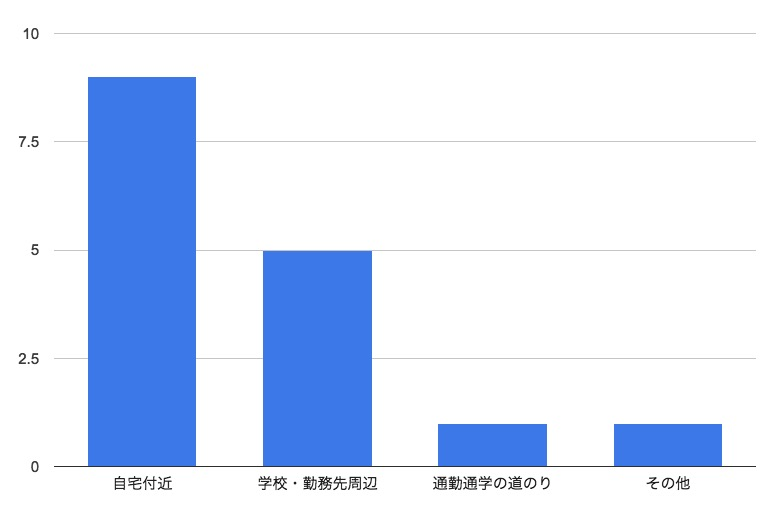
\includegraphics[width=0.8\hsize]{./images/curation_02_result.jpg}
      \caption{アンケート結果(設問2の回答結果)}
      \label{fig:curation_02_result}
    \end{center}
  \end{figure}
  \fi

  アプリを通じて,知ってよかった,行きたいと思った場所の情報についての回答内容として
  レストランやカフェ,ハンバーガー屋,ラーメン屋といったグルメスポットに関する情報が目立った.
  また「自宅付近ではあるが、普段の生活では行かない地域に美味しそうなカフェがあることを知り、行きたいと思った」「長年住んできた地元に自分の知らないオシャレなスポットがあることを知れたのが良かった。」
  などといった,
  生活圏内で今まで認知していなかったスポット情報を知れたという回答がいくつかみられた.
  また,これらの場所が自身の生活でどういった場所にあたるかの回答は
  自宅付近が64\%(9名),学校・勤務先周辺が35.7\%(5名),通勤・通学の道のり,その他がそれぞれ1名で,その他の内容は「出かけ先」であった.

  設問3の結果を図\ref{fig:curation_03_result}に,設問4の回答内容を表\ref{tab:curation-04-result}に示す.

  \fifigure
  \begin{figure}[H]
    \begin{center}
      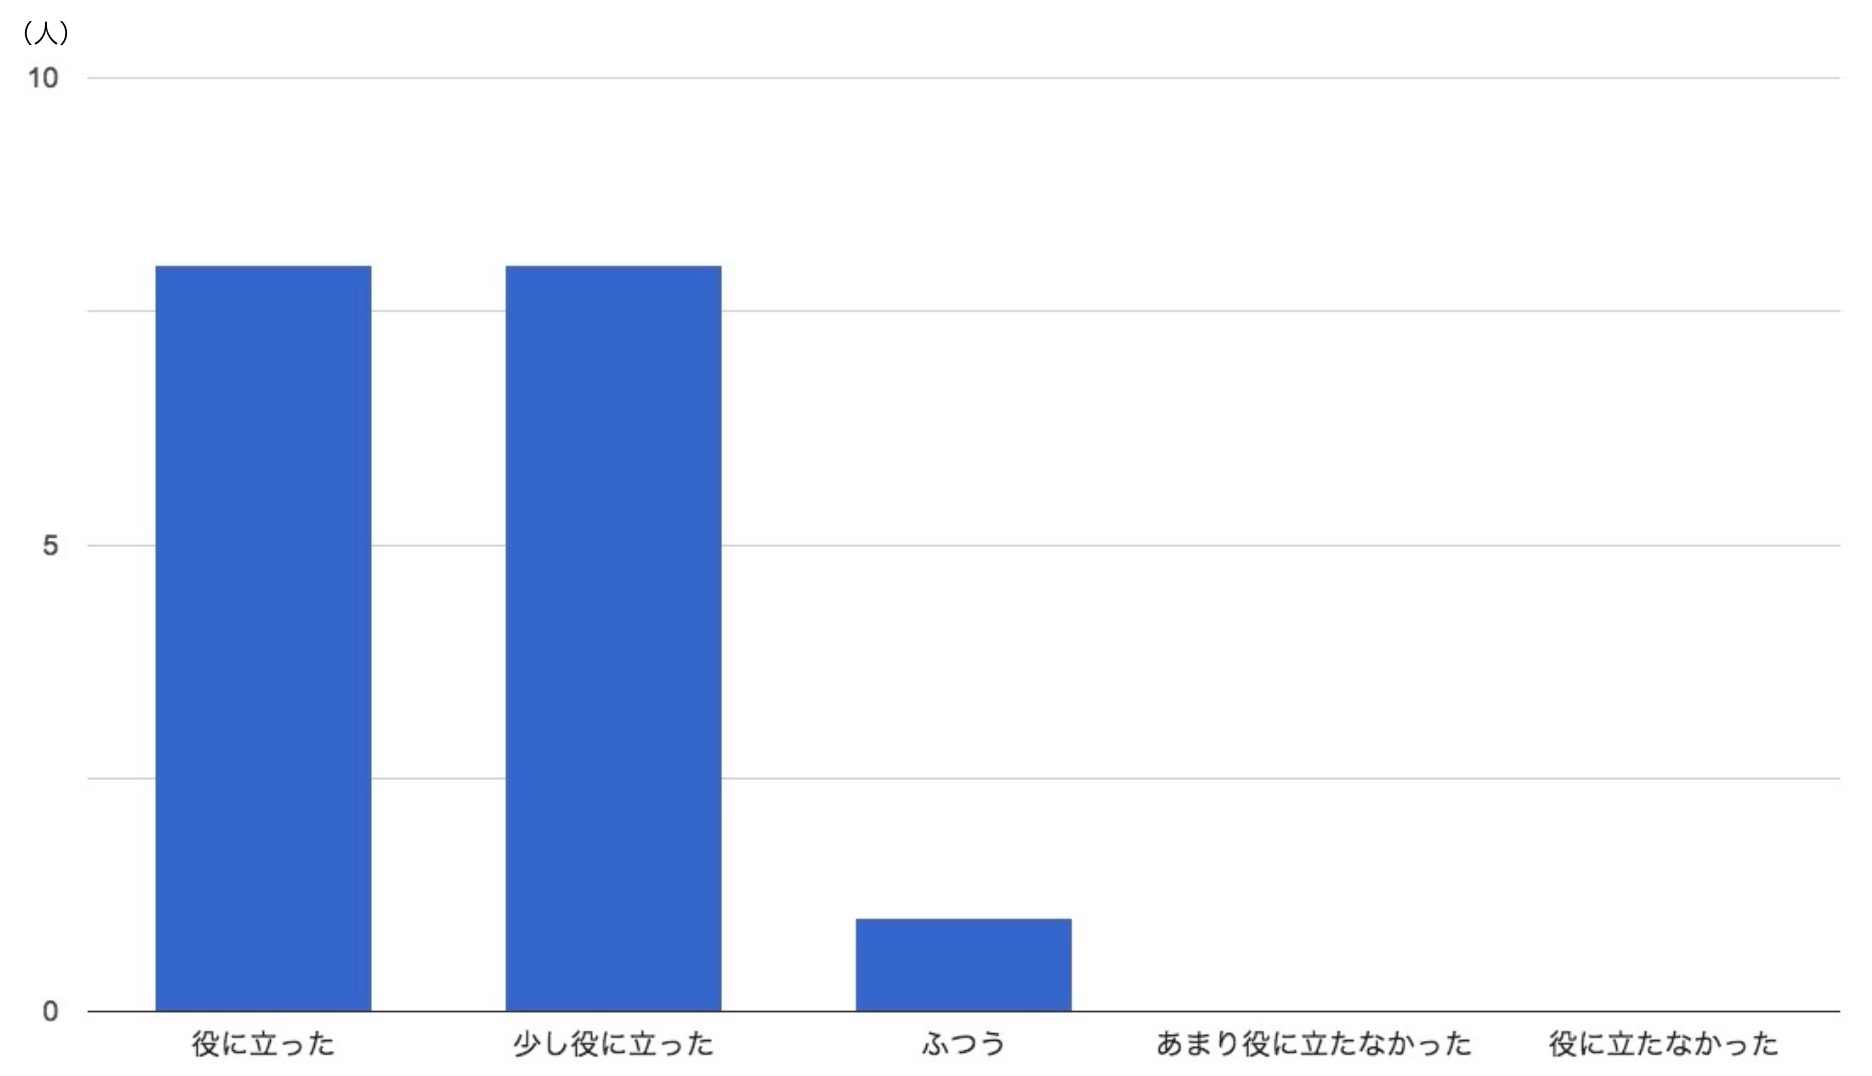
\includegraphics[width=0.8\hsize]{./images/curation_03_result.jpg}
      \caption{アンケート結果(設問3の回答内容)}
      \label{fig:curation_03_result}
    \end{center}
  \end{figure}
  \fi

  \begin{table}[H]
    \begin{center}
      \caption{アンケート結果(設問4の回答内容)}
      \renewcommand\arraystretch{1.2}
      \begin{tabular}{|p{15cm}|}
        \hline
        アプリで得た情報が役に立った,少し役に立った理由について \\
        \hline
        % 身の回りの情報って気がつかないことが多いから \\
        ・知らなかったところを知れました \\
        ・気軽に行けるところに素敵なお店があると知ると、生活が楽しくなるような気がする \\
        ・今までしらなかった場所や美味しそうなお店を知ることができた。 \\
        ・家の近くとか、よく行く場所の近くだから手軽にいきやすい感じがした \\
        ・通学に使う路線の沿線にある情報を一括で知ることができ、降りたことのない駅のことも知るきっかけになったから \\
        % メディアとしてまとめられているので情報がわかりやすかった \\
        ・普段キュレーションサイトなどを見ていて行きたいなと思っても、距離的になかなか機会が取れなかったりするので、このアプリは暇つぶしに見ていて良いと思ったときに気軽に行けるので良いなと思いました。 \\
        ・今までは調べる苦労からある程度場所を決めてから行くお店などを決めることが多かったのですが、このアプリは労力を使わずに行きたいところを絞れるので便利だと思いました。 \\
        ・ユーザーの興味や属性も考慮して情報をあげてもらえると嬉しいなーと。 \\
        ・期間限定の情報で、期間が終わってたこと \\
        % 面白そうなお店を知ることができた \\
        ・気になった所へ実際に足を運び、楽しく美味しい時間を過ごせたから。 \\
        ・最寄りの記事から出てきてくれるので、新しく生活圏の情報を得ることができました。 \\
        % 知らなかったお店があった \\
        ・今度行きたいと思える場所と出会えたので。ただ、まだ行っておらず本当によかったかはわからないので、役に立ったではなく、少し役に立ったにしている。 \\
        \hline
      \end{tabular}
      \label{tab:curation-04-result}
    \end{center}
  \end{table}

  アプリで得た情報が役に立ったかについての回答は「役に立った」が50\%(7名),「やや役に立った」が50\%(7名)であり,「ふつう」以下の回答は1名もいなかった.
  理由についての回答は
  設問1の回答内容に引き続き,今まで認知してなかった場所の情報を知れたことを評価する回答に加え,「気軽に行けるところに素敵なお店があると知ると、生活が楽しくなるような気がする」「家の近くとか、よく行く場所の近くだから手軽にいきやすい感じがした」といった,生活圏内のスポットであることから手軽に行けることを評価する回答が目立った.
  また,他の類似アプリやサービスと比較し,情報の探しやすさを評価する回答や,アプリで得た情報の場所に実際に足を運んだという回答もみられた.
  反対に「期間限定の情報で、期間が終わってた」という,記事内容の精度を指摘する回答がみられた.

  % 気軽に行けるのがよかった勢 1111
  % 知らなかったことが知れてよかった勢 1111
  % 他のアプリよりもよかったよ勢 11
  % 簡単に調べらるのがよかった勢 1
  % 身の回りの情報知れてよかった勢 11
  % 実際にその場所にいった勢 1
  % マイナスの意見 1


\end{enumerate}


\subsection{考察}
アプリの公開後のユーザを対象にしたアンケート調査の結果を元に,生活圏に基づいて情報の絞り込みを行う本アプリの利用可能性について考察する.

アプリを通して得たスポット情報が自身の生活でどういった場所にあたるかの回答においては,ほとんどが「自宅付近」もしくは「学校・勤務先周辺」と回答し「通勤通学の道のり」の割合は少なく,これは,生活圏を検出するシステムが移動経路の検出を考慮していなかったためだと考えられる.
アプリで得た情報の有用性に関する調査では,回答者14名のうち全員が「役に立った」または「やや役に立った」と回答し,手軽に利用できる生活圏内のスポット情報を得られたことや,身近の知らなかった情報を知れたことがその理由に多くあげられた.また,実際にその場所へ行った,もしくは行く予定を立てたという回答もいくつかみられた.
このことから,本アプリで用いたシステム及びインタフェースにより,
スポット情報を扱うWebメディアの情報が個々の生活圏に応じて最適化され,
ユーザは,距離的な障壁が低く手軽に利用可能な,日常生活において有用な情報を得られたといえる.
よって,パーソナライズの事例が多く見られる分野において,端末内に蓄積した位置情報を用いる新たな手法を創出できた.

一方,期間限定の情報を終了後にも関わらず提示してしまったことを踏まえ,プログラミングによる記事の選定の精度を向上させることが,本アプリにおける今後の課題であるといえる.
% 一方,インタフェースは既存のキュレーションアプリを参考に構成したため,特別インターフェースを評価する回答は見られなかった.
また,今回のアンケートでは回答者の属性が,20代や学生に偏ってしまったため,今後は多様なユーザを対象に調査する必要があるといえる.

\section{まとめ}
本章では,本研究の結論および研究成果が持つ意義,今後の課題と展望について述べる.

\subsection{本研究のまとめ}
本研究の目的は,端末内に蓄積された行動履歴をもとにWebサービスのパーソナライズを行うシステム・スマートフォンアプリを開発し,その利用可能性を示すことであった.
そのためにまず,スマートフォン内部に蓄積した位置情報をもとに,ユーザの生活圏を検出するシステムを構築した.
システムの精度を示した後,検出された生活圏に基づいて
1.全国のハザードマップの情報を絞り込んで提示するハザードマップアプリ,
2.スポット情報を扱うWebメディアの情報を絞り込んで提示するキュレーションアプリ
をそれぞれ開発し検証を行った.
その結果,
ハザードマップアプリでは,既存のアプリの操作性や閲覧性の低さといった課題を解決し,
キュレーションアプリでは,日常生活で有用な情報を個々に最適化し,パーソナライズの事例が多く見られる分野において,端末内に蓄積した位置情報を用いる新たな手法を創出できた.
% ハザードマップアプリでは,
% 国土数値情報が提供する全国のハザード情報オープンデータを
% アプリからAPI連携で利用可能になる設計をし,
% 全国のハザード情報の中から,個々のユーザの生活圏に基づいて収集し,
% 提示するアプリケーションを開発した.
% 実際にアプリをユーザに使ってもらい検証を行なった
% 結果
% 本アプリの
% インタフェースデザインとシステムによる
% 高いユーザビリティと,閲覧性?を得られ,
% 既存のハザードマップアプリの閲覧性の低さを解決した
%
% 過半数のユーザが本アプリを「使いやすい」と回答し,絞り込まれた情報の見やすさやインターフェースデザインの評価がその理由にあげられた.
% 本アプリで用いたシステム及びインタフェースが,ハザードマップの情報の閲覧性やアプリのユーザビリティを向上させる要因になったといえる.
% 検出された生活圏に基づき,ハザードマップの情報を絞り込んでユーザに提示する本手法により,既存のハザードマップアプリの操作性・閲覧性の低さを解決できたといえる。
%
%
% キュレーションアプリでは,
% インターネット上に散在するWebメディアの中から,
% スポット情報を扱うメディアから
% 生活圏に基づいてデータを収集し提示するアプリケーションを開発した
% 〜で検証を行なった
% 結果
%
%
% 日常生活で有用な情報を個々に最適化できたとことを確認できた

以上の成果により,
% 端末内に蓄積させた行動履歴をもとにWebサービスのパーソナライズを行う本アプリの,
ハザードマップアプリとキュレーションアプリの二つの領域において,本手法を用いたパーソナライズを行うスマートフォンアプリを開発し,その利用可能性を示した.

本研究の貢献は,スマートフォンに蓄積させたデータを活用し,様々な情報を適切に絞り込んで,Webサービスのパーソナライズを行うシステム及びスマートフォンアプリを開発し,その利用可能性を示したことである.このことによって,今後も社会に浸透していくことが予想される携帯端末を用いて,膨大な情報を扱うWebサービスのユーザ体験を向上させるための一つのモデルを示すことができた.


\subsection{今後の課題と展望}
本研究では,高頻度で訪れる地域をユーザの生活圏として検出し,一定範囲内のエリアに基づいて情報の絞り込みを行なったが,
松尾ら,宮崎らの,各エリアを繋ぐ経路をユーザの生活圏として検出する技術\cite{matsuo}\cite{docomo}を用いて情報を収集する手法も検討できる.
これによりユーザは,通勤通学の道のりや乗り換えの駅など,日常の移動で利用するが活用度の低い場所の情報が得られると考えられる.
本研究のハザーマップアプリにおいては,普段の移動中にも起こりうる災害のリスク・対策を,事前に素早く学ぶことができると予想できる.
スポット情報を扱うキュレーションアプリにおいては,度々通過するが活用することのなかった場所の有用な情報を得られ,より新しい発見を促すことができると予想できる.
また宮崎らの,蓄積した過去の位置情報からその後の行動を推定する技術\cite{docomo}を用いれば,
よりユーザの生活スタイルに合わせた情報提示,サービス提供が可能になると考える.加えて,オンライン上の行動データを組み合わせることでの展開性も考えられる。
このように,蓄積された位置情報を用いたWebサービスのパーソナライズには様々な展開の余地があるといえる.
しかし,大規模なデータ分析を行うには端末内での処理容量に限界があるため,検出精度との兼ね合いや,外部サーバとの連携・プライバシー保護のための施策を考える必要があるといえる.
また,高度な検出には,短間隔かつ高精度の位置情報取得が求めらるため,スマートフォンアプリにおいては電池消費が懸念されるという課題もある.

本研究では位置情報履歴から生活圏を割り出すことによるパーソナライズを行なったが,今後はこれらの課題を踏まえつつ,ユーザの多様な行動分析を行い,より細やかなパーソナライズの手法と,その利用可能性を検討していく.

\newpage
\section*{謝辞}
本研究を進めるにあたり,指導教官として適切なご指導と助言いただきました,渡邉英徳先生に謹んで感謝の意を表します.
また,笠原信一先生,並びに,楠見清先生には副査としてご助言を戴くとともに本論文の細部にわたりご指導を戴き,ここに深く感謝の意を表します.

防災アプリの実証実験の実施においては,国土交通省国土地理院応用地理部防災アプリ事務局,株式会社パスコの皆様にご尽力を賜りました.深く感謝申し上げます.
また,ハザードマップアプリ共同開発者の木村汐里さん,WEBアンケート調査にご協力いただいた皆様に,謹んで御礼申し上げます.
最後に,日常の議論を通じて多くの知識や示唆を頂いた渡邉英徳研究室の皆様に深く感謝致します.

% 横根集落の活動にあたり,ご尽力いただきました魚沼市の佐藤陽二さん,魚沼市地域おこし協力隊の大野久美子さんにも深く御礼申し上げます.
% 最後に,本研究を支え,日常の議論を通じて多くの知識や示唆を頂いたネットワークデザインスタジオのみなさんに深く感謝致します.

\newpage


\begin{thebibliography}{999}
\bibitem{izumi}
  泉浩人:
  競争戦略としてのユーザーエクスペリエンスデザイン - 「買い手市場」を勝ち抜くためのヒント,
  情報管理2016.11. vol.59 no.8,
  pp.535-543
  2016
\bibitem{okunuki}
  奥貫泰正:
  新しい企業・経営像と経営診断のパラダイム・シフト - マーケティング行動における定性的評価基準の必要性 -,
  2010
\bibitem{mochimaru}
  持丸正明:
  人間中心設計はICT/RTと融合し社会共有価値を目指す,
  日本ロボット学会誌 Vol.32 No.10,
  pp.884-846,
  2014
\bibitem{tameco}
  タメコ株式会社,株式会社博報堂DYメディアパートナーズ,デジタル・アドバタイジング・コンソーシアム株式会社:
  生活者のリアル行動特性に基づきパーソナライズされたメディアサービスの提供に向けた取り組みを開始,
  2016
\bibitem{bitblend}
  株式会社サイバーエージェント:
  BitBlend,

  https://www.cyberagent.co.jp/newsinfo/info/detail/id=11495
\bibitem{matsuo}
  松尾雄二,原直,阿部匡伸:
  滞在地と経路に着目した生活圏抽出法の検討,
  情報処理学会第76回全国大会,
  pp.37-38
  2014
\bibitem{docomo}
  宮崎雄一郎,山田直治,住谷哲夫,磯田佳徳:
  ユーザの行動に合わせたサービス実現のための行動推定技術の開発,
  NTT Docomo テクニカル・ジャーナル Vol.17 No.3,
  pp.55-61,
  2009
% \bibitem{amazon}
%   Amazon.com:
%   Amazon,
%   https://www.amazon.co.jp/
\bibitem{mail_publisher_smart}
  エクスペリアンジャパン:
  MailPublisher Smart,
  
  https://www.marketinggate.jp/service/system/MPSE/
\bibitem{mail_publisher_smart_study}
  Marketing Land:Study: Personalized Emails Deliver 6X Higher Transaction Rates, But 70\% Of Brands Fail To Use Them,
  http://marketingland.com/study-70-brands-personalizing-emails-missing-higher-transaction-rates-revenue-73241,
  2013
\bibitem{yahoo}
  ヤフー株式会社:
  Yahoo!防災速報,
  https://emg.yahoo.co.jp/
\bibitem{watav}
  アライドアーキテクツ株式会社:
  watav,
  http://watav.com/
\bibitem{ohmukai}
  大向一輝,国立情報学研究所:
  SNSの歴史,
  通信ソサイエティマガジン No.34,
  pp.70-75,
  2015
  http://watav.com/
\bibitem{sample}
  著者名1,著者名2
  論文タイトル名、
  発表シンポジウム・会議名、
  発表学会名、
  記事番号やページ、
  発表年

\end{thebibliography}


\end{document}
